% !TEX program = lualatex
\documentclass[8pt,t,aspectratio=169]{beamer}

\usepackage{fontspec}
\usepackage{amsmath,amssymb}
\usepackage{tikz}

\setsansfont{Noto Sans}[
  Language       = Bulgarian,
  Script         = Cyrillic
]

% Fonts
\setbeamerfont{title}{series=\bfseries, size={\fontsize{14}{14}\selectfont}}
\setbeamerfont{subtitle}{series=\mdseries, size={\fontsize{9}{9}\selectfont}}
\setbeamerfont{frametitle}{series=\bfseries, size={\fontsize{9}{9}\selectfont}}
\setbeamerfont{framesubtitle}{series=\mdseries, size={\fontsize{9}{9}\selectfont}}
\setbeamerfont{normal text}{size={\fontsize{7}{7}\selectfont}}
\setbeamerfont{block body}{size={\fontsize{7}{7}\selectfont}}
\setbeamerfont{block title}{size={\fontsize{9}{9}\selectfont}}

% Colors
\definecolor{DarkBlue}{RGB}{0, 32, 96}
\definecolor{DarkGray}{rgb}{0.50,0.50,0.50}

\setbeamercolor{block title}{fg=DarkBlue}
\setbeamercolor{frametitle}{fg=DarkBlue}
\setbeamercolor{framesubtitle}{fg=DarkGray}
\setbeamercolor{title}{fg=DarkBlue}
\setbeamercolor{subtitle}{fg=DarkGray}

% Footline
\setbeamertemplate{footline}{
  \begin{beamercolorbox}[wd=\paperwidth, dp=1ex, rightskip=4ex]{footline_container}%
    \hfill
    \usebeamercolor[fg]{page number in head/foot}
    \usebeamerfont{page number in head/foot}
    \insertframenumber{} / \inserttotalframenumber
  \end{beamercolorbox}
  
  \vspace*{1ex}

  \begin{beamercolorbox}[wd=\paperwidth, ht=0.4ex, dp=0pt]{footline_stripe}%
    \colorbox{DarkBlue}{\rule{\paperwidth}{0.4ex}}%
  \end{beamercolorbox}
}

% Center title page
\setbeamertemplate{title page}{
  \vfill
  \centering
  \usebeamerfont{title}\usebeamercolor[fg]{title}\inserttitle\par
  \vspace{0.5em}
  \usebeamerfont{subtitle}\usebeamercolor[fg]{subtitle}\insertsubtitle\par
  \vfill
}

% Use circle bullets for itemize lists
\setbeamertemplate{items}[circle]

% Remove navigation symbols
\setbeamertemplate{navigation symbols}{}

% Small left/right margins
\setbeamersize{text margin left=0.5cm, text margin right=0.5cm}

\setbeamertemplate{frametitle}{} % Изчистване на стандартното заглавие

% Auto numbering for sections and subsections
\setbeamertemplate{section in toc}[sections numbered]
\setbeamertemplate{subsection in toc}[subsections numbered]
\setbeamertemplate{frametitle}{} % Изчистване на стандартното заглавие

% 1. Предефинираме формата на \thesubsection, така че \ref да връща Секция.Подсекция (напр. 1.1)
\renewcommand{\thesubsection}{\thesection.\arabic{subsection}.}
\renewcommand{\thesubsubsection}{\arabic{subsubsection}.}

% 2. Нова команда за автоматично слагане на "Виж" и скоби
\newcommand{\secref}[1]{(Виж секция \ref{#1})}

\setbeamertemplate{headline}{%
  \ifnum\thepage>1
    \vspace*{0.3cm}
    \begin{beamercolorbox}[wd=\paperwidth,ht=3.2ex,dp=1.2ex,leftskip=0.5cm,rightskip=0.5cm]{frametitle}%
      \usebeamerfont{frametitle}
      \ifx\insertsubsubsectionhead\empty
        \ifx\insertsubsectionhead\empty
          \thesection~\insertsectionhead
        \else
          \thesubsection~\insertsubsectionhead  % <-- ТУК: \thesubsection вече е "1.1"
        \fi
      \else
        \thesubsection\thesubsubsection~\insertsubsubsectionhead
      \fi
    \end{beamercolorbox}%
    \vspace*{0.05cm}%
  \fi
}

% --------------------------------------------------------------------------------

\title{Многомерна статистика}
\subtitle{Многомерни методи за статистическо моделиране}
\date{}

% --------------------------------------------------------------------------------

\begin{document}
\setcounter{section}{-1}
% --------------------------------------------------------------------------------

\begin{frame}[c]
    \titlepage
\end{frame}

% --------------------------------------------------------------------------------

\section{Въведение}
\subsection{За мен}

% --------------------------------------------------------------------------------

\begin{frame}
  \begin{columns}[c]
    \begin{column}{0.75\textwidth}
      \begin{itemize}
        \item 2017-2022
          \begin{itemize}
            \item Магистър - Бизнес инженер - специалност Анализ Данни
            \item Гентски Университет, Белгия
            \item Икономически факултет
          \end{itemize}
      \end{itemize}
    \end{column}
    \begin{column}{0.25\textwidth}
      \centering
      
\includegraphics[width=0.7\linewidth, height=1.2cm, keepaspectratio]{logo_ugent.png}
    \end{column}
  \end{columns}

  \vspace{0.2cm}

  \begin{columns}[c]
    \begin{column}{0.75\textwidth}
      \begin{itemize}
        \item 2022-2026
          \begin{itemize}
            \item Софтуерен инженер
            \item BrightAnalytics (финтек компания)
            \item Автоматизация на счетоводни и оперативни доклади
            \item Бекенд архитектура, оптимизация на фонови процеси, синхронизация на данни и приложения на изкуствен интелект
          \end{itemize}
      \end{itemize}
    \end{column}
    \begin{column}{0.25\textwidth}
      \centering
      
\includegraphics[width=0.7\linewidth, height=1.2cm, keepaspectratio]{logo_bright.png}
    \end{column}
  \end{columns}

  \vspace{0.2cm}

  \begin{columns}[c]
    \begin{column}{0.75\textwidth}
      \begin{itemize}
        \item 2026-*
          \begin{itemize}
            \item Асистент и докторант в ТУ
            \item Катедра информатика
            \item Програмиране, многомерна статистика, квантова информатика
          \end{itemize}
      \end{itemize}
    \end{column}
    \begin{column}{0.25\textwidth}
      \centering
      
\includegraphics[width=0.7\linewidth, height=1.2cm, keepaspectratio]{logo_tu.png}
    \end{column}
  \end{columns}
\end{frame}

% --------------------------------------------------------------------------------

\subsection{За курса}

% --------------------------------------------------------------------------------

\begin{frame}
  \small
  Накратко:
  \begin{itemize}
    \item Надграждане на вече усвоени умения за многомерен анализ
    \item Основи на статистическо моделиране и машинно самообучение
    \item Приложения и визуализации в Python
  \end{itemize}
  Теми:
  \begin{enumerate}
    \item Интродукция в статистическото моделиране, метрики и валидация
    \item Линейно моделиране: обобщен линеен модел, пробит и лог-линеен модел
    \item Основи за класификация: ковариационна матрица, разстояние на Махаланобис, рангова корелация, частна и множествена корелация, канонична корелация
    \item Линеен и нелинеен дискриминантен анализ
    \item Дървовидни модели: класификационни и регресионни дървета
    \item Клъстерен анализ и йерархичен клъстерен анализ
    \item Метод на главните компоненти и многомерно скалиране
    \item Факторен, кореспондентен и латентен семантичен анализ
  \end{enumerate}
\end{frame}

% --------------------------------------------------------------------------------

\section{Интродукция в статистическото моделиране, метрики и валидация}

\subsection{Статистическо моделиране}

% --------------------------------------------------------------------------------

\begin{frame}
  \begin{itemize}
    \item Есенция на статистическото моделиране. Истинска функция $f$, с нормално разпределен шум
    
      \[ \mathbf{Y} = f(\mathbf{X}) + \epsilon \quad \epsilon \sim \mathcal{N}(0, \sigma^2) \]

    \vspace{0.5ex}

    \item Разпределение на $\mathbf{Y} \ | \ \mathbf{X}$
    
      \[ \mathbf{Y} \ | \ \mathbf{X} \sim \mathcal{N}(f(\mathbf{X}), \sigma^2) \]
  \end{itemize}

  \vspace{1ex}
  \centering
  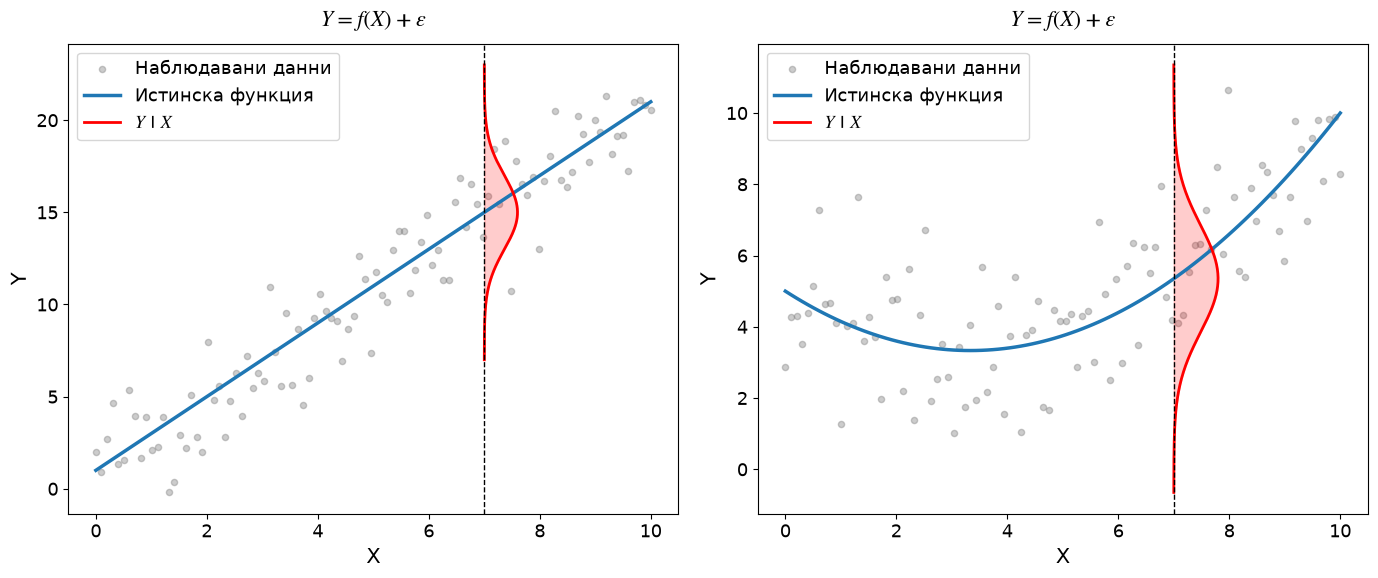
\includegraphics[width=0.8\textwidth]{images/true_function_with_normal_error.png}
\end{frame}

% --------------------------------------------------------------------------------

\begin{frame}
  \begin{columns}[T]
    \begin{column}{0.35\textwidth}
      \begin{itemize}
        \item Оценяване на $f(\mathbf{X})$

        \vspace{1ex}

        \qquad $\hat{\mathbf{Y}} = \hat{f}(\mathbf{X})$

        \vspace{1ex}

        \item Очаквана стойност на оценената функция (модел)
        
        \vspace{1ex}

        \qquad $\mathbb{E}[\hat{f}(\mathbf{X})]$

        \vspace{1ex}

        \item Вариация на оценената функция (модел)
        
        \vspace{1ex}
        
        \qquad $\text{Var}[\hat{f}(\mathbf{X})]$
      \end{itemize}
    \end{column}

    \begin{column}{0.65\textwidth}
      \centering
      \includegraphics[width=\textwidth]{images/expected_value_and_theoretical_variance.png}
    \end{column}
  \end{columns}
\end{frame}

% --------------------------------------------------------------------------------

\subsection{Систематична грешка и вариация}
\label{subsection:систематична_грешка_и_вариация}

% --------------------------------------------------------------------------------

\begin{frame}
  \begin{itemize}
    \item Систематична грешка, вариация и неотстранима грешка
    
      \begin{align*}
        \mathbb{E}\left[(\mathbf{Y} - \hat{\mathbf{Y}})^2\right] &= \mathbb{E}\left[\mathbf{Y} - \hat{\mathbf{Y}}\right]^2 + \text{Var}\left[\mathbf{Y} - \hat{\mathbf{Y}}\right] \\
        &= \mathbb{E}\left[f(\mathbf{X}) + \epsilon - \hat{f}(\mathbf{X})\right]^2 + \text{Var}\left[f(\mathbf{X}) + \epsilon - \hat{f}(\mathbf{X})\right] \\
        &= \underbrace{\left(f(\mathbf{X}) - \mathbb{E}\left[\hat{f}(\mathbf{X})\right]\right)^2}_{\text{Bias}^2} + \underbrace{\text{Var}\left[\hat{f}(\mathbf{X})\right]}_{\text{Variance}} + \underbrace{\vphantom{\left(f(\mathbf{X})\right)^2}\sigma^2}_{\text{Irreducible error}}
      \end{align*}
  \end{itemize}
\end{frame}

% --------------------------------------------------------------------------------

\begin{frame}
  \centering
  \small
  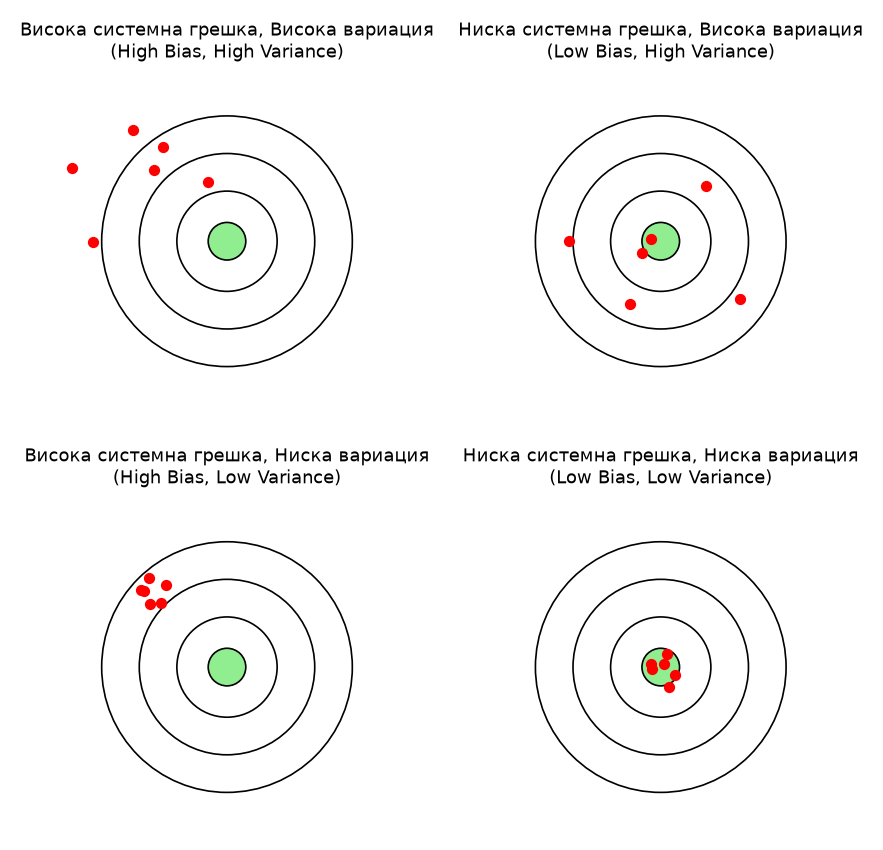
\includegraphics[width=0.55\textwidth]{images/bullseye_bias_variance.png}
\end{frame}

% --------------------------------------------------------------------------------

\subsubsection{Баланс между систематична грешка и вариация (bias-variance tradeoff)}
% --------------------------------------------------------------------------------

\begin{frame}
  \begin{itemize} 
    \item Простите модели имат висока систематична грешка, но ниска вариация
    \item Гъвкавите модели имат ниска систематична грешка, но висока вариация
  \end{itemize}
  
  \centering
  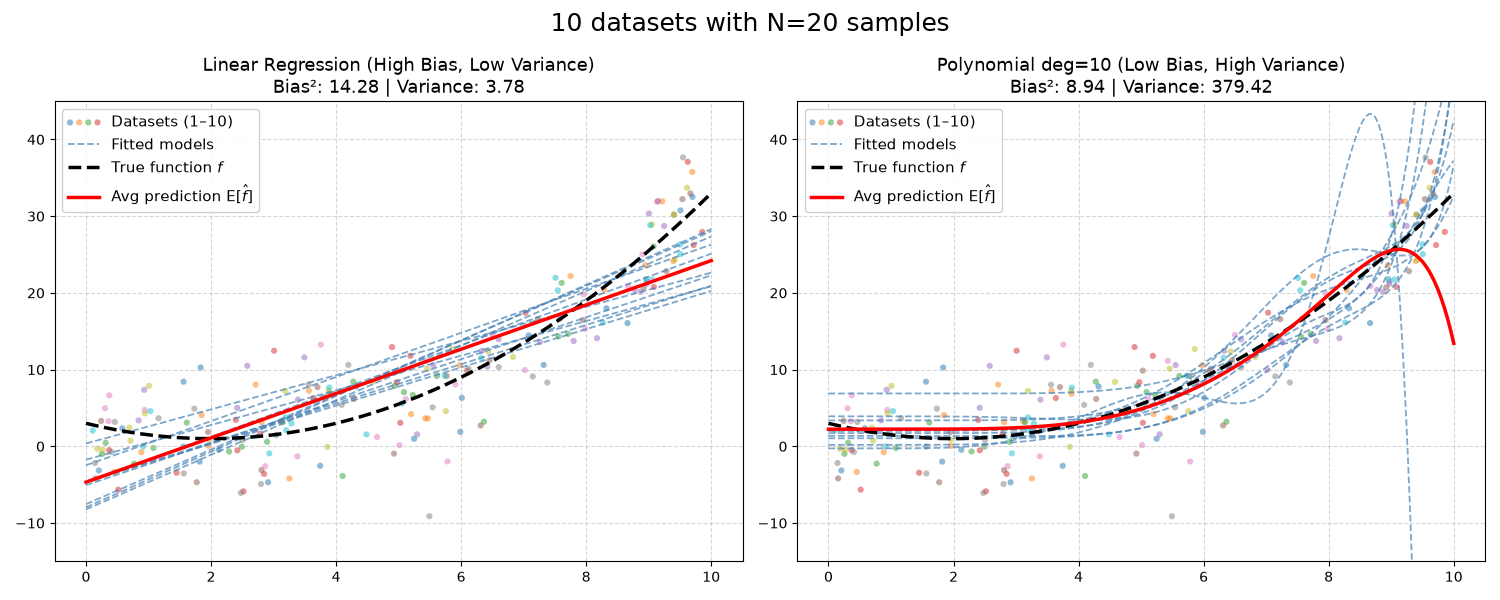
\includegraphics[width=\textwidth]{images/bias_variance_tradeoff_n_20.png}
\end{frame}

% --------------------------------------------------------------------------------

\begin{frame}
  \begin{itemize}
    \item При наличие на повече данни вариацията на модела намалява

    \vspace{1ex}

    \qquad $\textsf{Var}[\bar{\mathbf{Y}} | \mathbf{X}] = \frac{\sigma^2}{\text{N}}$
    
  \end{itemize}
  
  \centering
  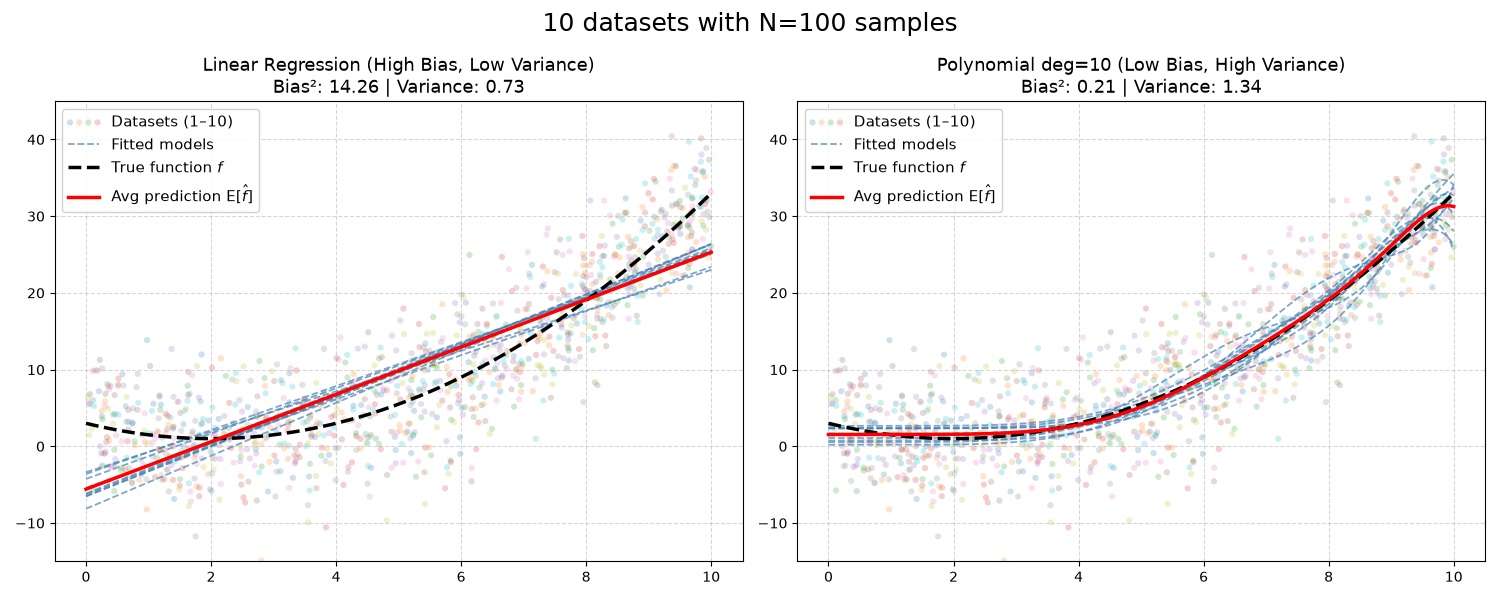
\includegraphics[width=\textwidth]{images/bias_variance_tradeoff_n_100.png}
\end{frame}

% --------------------------------------------------------------------------------

\begin{frame}
  \begin{itemize}
    \item Не винаги е възможно да набавим повече данни или да опростим модела!!!
  \end{itemize}

  \centering
  \small
  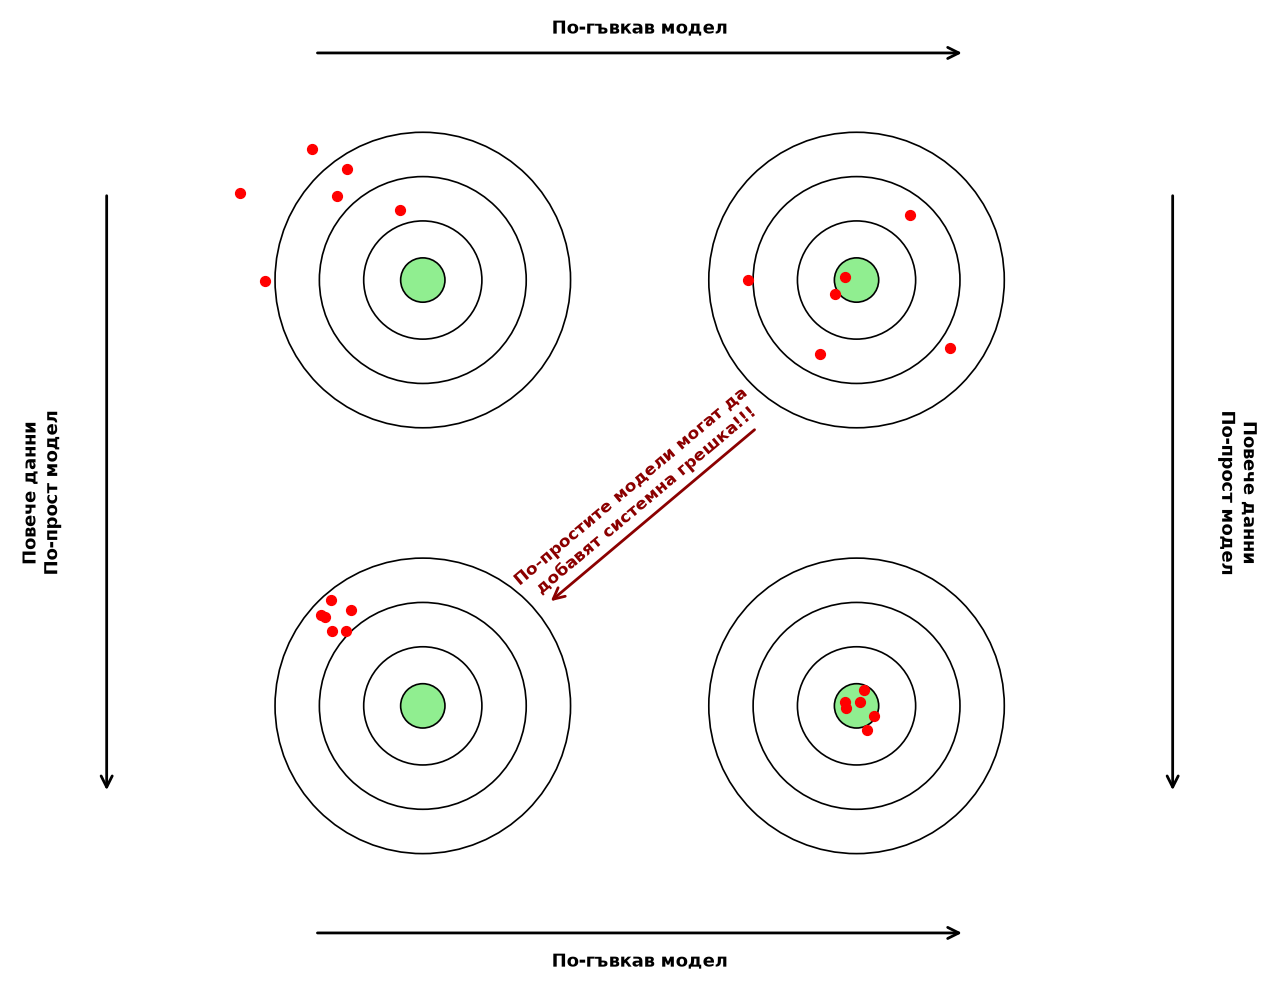
\includegraphics[width=0.58\textwidth]{images/bullseye_bias_variance_with_conclusion.png}
\end{frame}

% --------------------------------------------------------------------------------

\subsection{Видове статистическо обучение}

% --------------------------------------------------------------------------------

\begin{frame}
  \begin{itemize}
    \item Насочено обучение (supervised learning)\\
      {\small\itshape\color{gray} (налична целева променлива)}
    \item Ненасочено обучение (unsupervised learning)\\
      {\small\itshape\color{gray} (налични само независими променливи)}
  \end{itemize}
\end{frame}

% --------------------------------------------------------------------------------

\begin{frame}
  \begin{columns}[T]
    \begin{column}[T]{0.52\textwidth}
      \begin{itemize}
        \item Насочено обучение
        \begin{itemize}
          \item Регресия
          \begin{itemize}
            \item Непрекъсната целева променлива\\
            \vspace{1ex}
              {\small\itshape\color{gray} (напр. височина, тегло)}
            \vspace{1ex}
            \item Дискретна целева променлива\\
            \vspace{1ex}
              {\small\itshape\color{gray} (напр. бройки)}
            \vspace{1ex}
            \item Ординална целева променлива\\
            \vspace{1ex}
              {\small\itshape\color{gray} (напр. лошо, средно, отлично)}
            \vspace{0.5ex}
            \item Моделираната величина е непрекъсната, дискретна или ординална\\
            \vspace{1ex}
              {\small\itshape\color{gray} (напр. \textbf{логистичната регресия} прогнозира вероятности, въпреки че целевата променлива е номинална и се използва за класификация)}
            \vspace{1ex}
          \end{itemize}
        \end{itemize}
      \end{itemize}
    \end{column}

    \begin{column}[T]{0.48\textwidth}
      \centering
      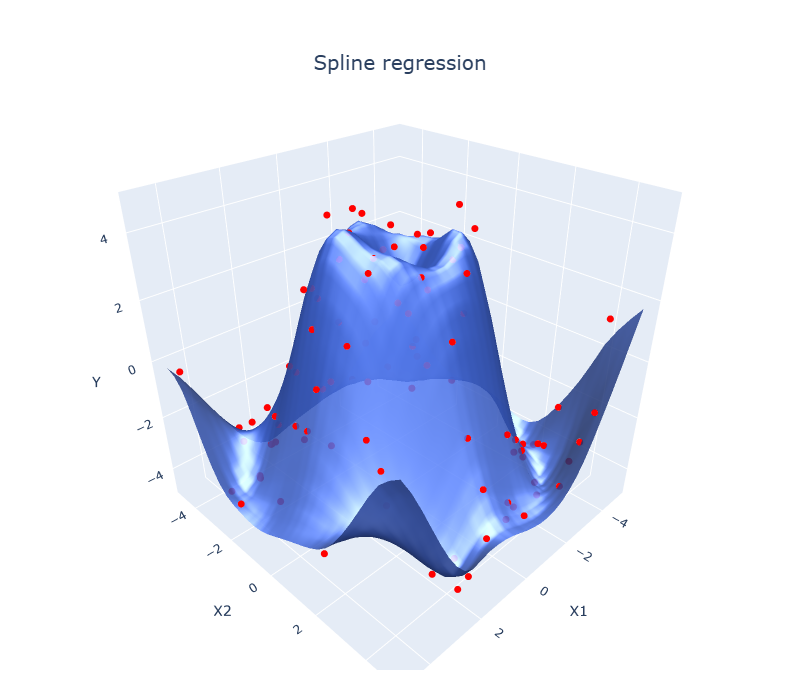
\includegraphics[width=\textwidth]{images/3d_spline.png}
    \end{column}
  \end{columns}
\end{frame}

% --------------------------------------------------------------------------------

\begin{frame}
  \begin{columns}[T]
    \begin{column}[T]{0.54\textwidth}
      \begin{itemize}
        \item Насочено обучение
        \begin{itemize}
          \item Класификация
          \begin{itemize}
            \item Бинарна целева променлива\\
            \vspace{1ex}
              {\small\itshape\color{gray} (напр. спам / не е спам, 0 / 1)}
            \vspace{1ex}
            \item Многокласова целева променлива\\
            \vspace{1ex}
              {\small\itshape\color{gray} (напр. куче / котка / птица)}
            \vspace{1ex}
          \end{itemize}
        \end{itemize}
      \end{itemize}
    \end{column}

    \begin{column}[T]{0.46\textwidth}
      \centering
      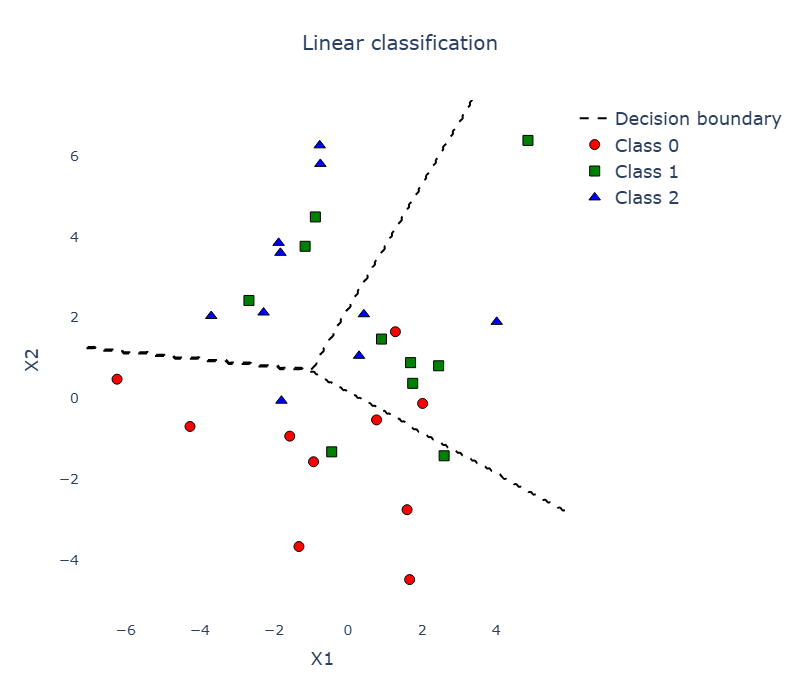
\includegraphics[width=\textwidth]{images/classification_boundaries.png}
    \end{column}
  \end{columns}
\end{frame}

% --------------------------------------------------------------------------------

\begin{frame}
  \begin{itemize}
    \item Ненасочено обучение
    \begin{itemize}
      \item Клъстеризация\\
      \vspace{0.5ex}
      {\small\itshape\color{gray} (напр. групиране на клиенти или демографски групи по поведение)}\\
      \vspace{1ex}
    \end{itemize}
  \end{itemize}
  \centering
  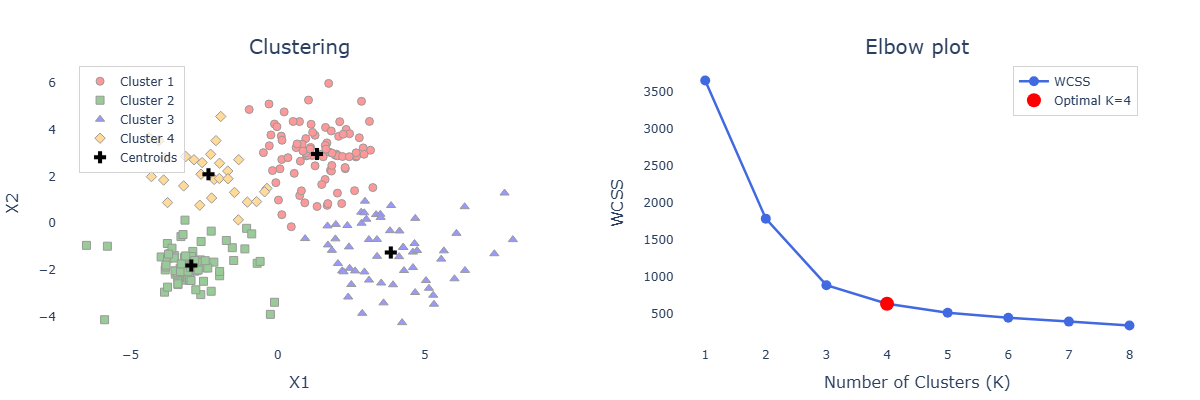
\includegraphics[width=0.9\textwidth]{images/clustering_with_scree.png}
\end{frame}

% --------------------------------------------------------------------------------

\begin{frame}
  \begin{itemize}
    \item Ненасочено обучение
    \begin{itemize}
      \item Намаляване на размерността\\
      \vspace{0.5ex}
      {\small\itshape\color{gray} (напр. за опростяване на модела, подбор на най-важните характеристики или елиминиране на зависимостите между променливите)}\\
      \vspace{1ex}
    \end{itemize}
  \end{itemize}
  \centering
  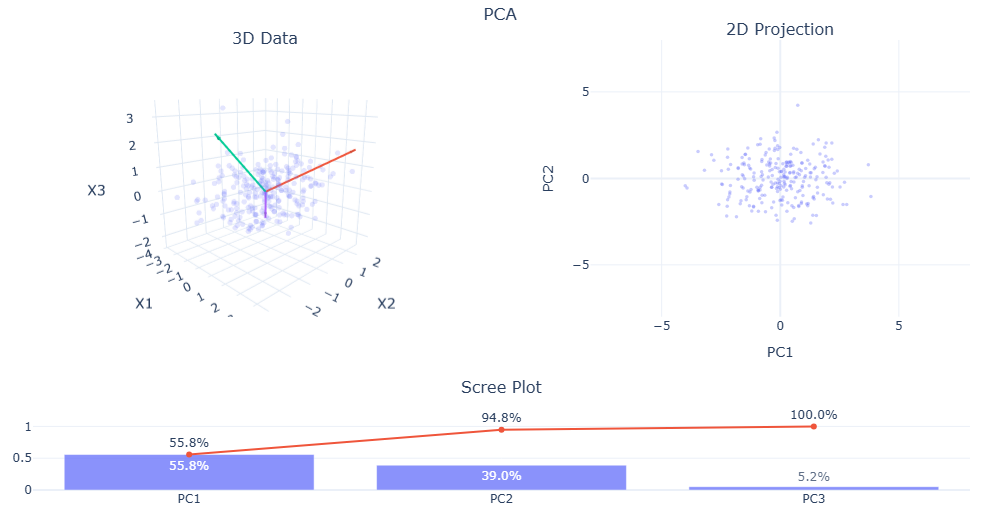
\includegraphics[width=0.8\textwidth]{images/pca.png}
\end{frame}

% --------------------------------------------------------------------------------

\begin{frame}
  \begin{itemize}
    \item Ненасочено обучение
    \begin{itemize}
      \item Генеративни модели\\
      {\small\itshape\color{gray} (напр. синтез на данни)}\\
      \vspace{1ex}
      \item Автоенкодери\\
      {\small\itshape\color{gray} (напр. използване на автоенкодери за намаляване на размерността)}\\
      \vspace{1ex}
      \item ...
    \end{itemize}
  \end{itemize}
  \centering
\end{frame}

% --------------------------------------------------------------------------------

\subsection{Метрики}

% --------------------------------------------------------------------------------

\begin{frame}[t]
  \begin{itemize}
    \item Как оценяваме грешката на модела?
    \begin{itemize}
      \item \textbf{Избор на метрика}
      \item Метод на валидация
    \end{itemize}
  \end{itemize}

  \vspace{0.1cm}

  \begin{columns}[c, onlytextwidth]
    \begin{column}{0.7\textwidth}
      \begin{itemize}
        \item Метрики за регресия:
      \end{itemize}

      \hspace*{1.5em}
      \begin{minipage}{0.75\linewidth}
        \small
        \begin{alignat*}{2}
          \text{MSE} &= \frac{1}{\mathsf{N}}\sum_{i}^{\mathsf{N}}(y_i - \hat{y}_i)^2 && \quad [\text{unit}^2] \\[6pt]
          \text{RMSE} &= \sqrt{\text{MSE}} && \quad [\text{unit}] \\[6pt]
          \text{MAE} &= \frac{1}{\mathsf{N}}\sum_{i}^{\mathsf{N}}|y_i - \hat{y}_i| && \quad [\text{unit}] \\[6pt]
          \text{MAPE} &= \frac{100\%}{\mathsf{N}}\sum_{i}^{\mathsf{N}}\frac{|y_i - \hat{y}_i|}{y_i} && \quad [\% \text{ units}] \\[6pt]
          R^2 &= 1 - \frac{\sum_{i}^{\mathsf{N}}(y_i - \hat{y}_i)^2}{\sum_{i}^{\mathsf{N}}(y_i - \bar{y})^2} && \quad [\% \text{ обяснена вариация}]
        \end{alignat*}
      \end{minipage}
    \end{column}
  \end{columns}

  \begin{tikzpicture}[remember picture, overlay]
    \node[anchor=east] at ([xshift=-0.15cm, yshift=1cm]current page.east) {
      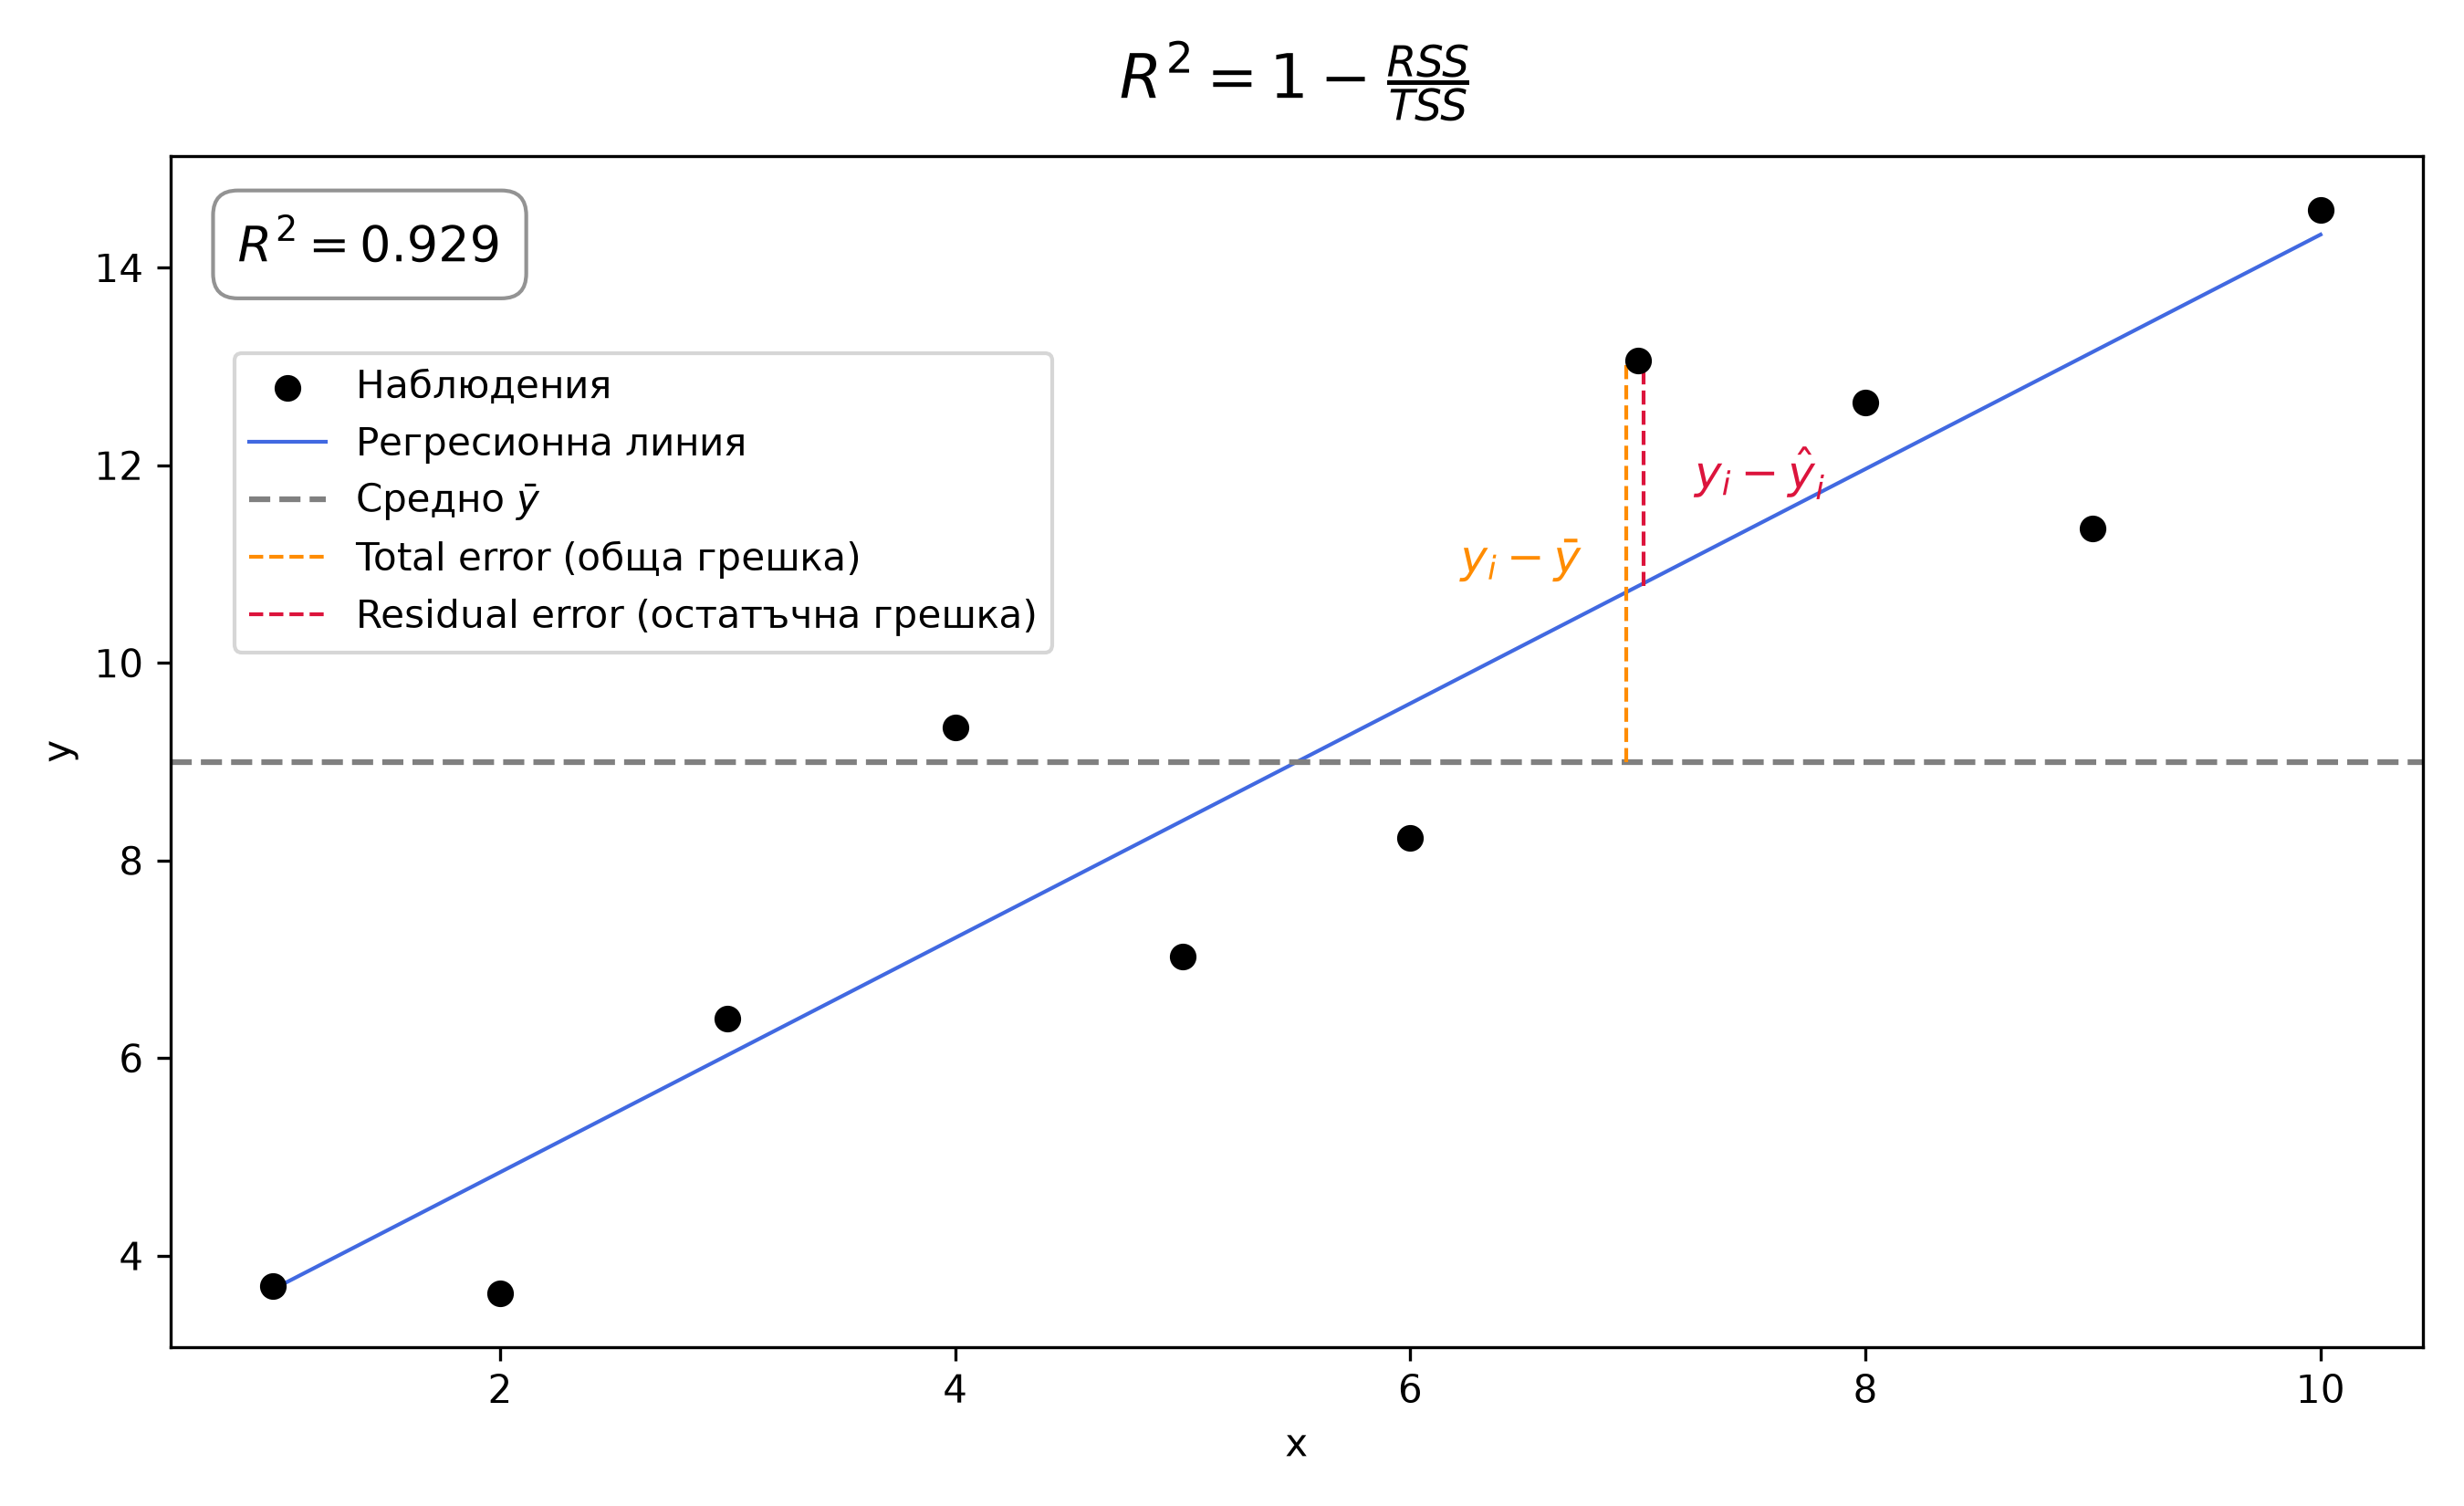
\includegraphics[width=0.55\paperwidth]{images/interpretation_r_squared.png}
    };
  \end{tikzpicture}
\end{frame}

% --------------------------------------------------------------------------------

\begin{frame}[t]
  \begin{itemize}
    \item Как оценяваме грешката на модела?
    \begin{itemize}
      \item \textbf{Избор на метрика}
      \item Метод на валидация
    \end{itemize}
  \end{itemize}

  \vspace{0.1cm}

  \begin{columns}[c, onlytextwidth]
    \begin{column}{0.4\textwidth}
      \begin{itemize}
        \item Метрики за регресия с чувствителност към аномалии:
      \end{itemize}

      \hspace*{1.5em}
      \begin{minipage}{0.85\linewidth}
        \small
        \begin{align*}
          {\color{red}\text{MSE}}\\[6pt]
          {\color{red}\text{RMSE}}\\[6pt]
          {\color{red}R^2}
        \end{align*}
      \end{minipage}
    \end{column}

    \begin{tikzpicture}[remember picture, overlay]
      \node[anchor=east] at ([xshift=-0.15cm, yshift=1cm]current page.east) {
        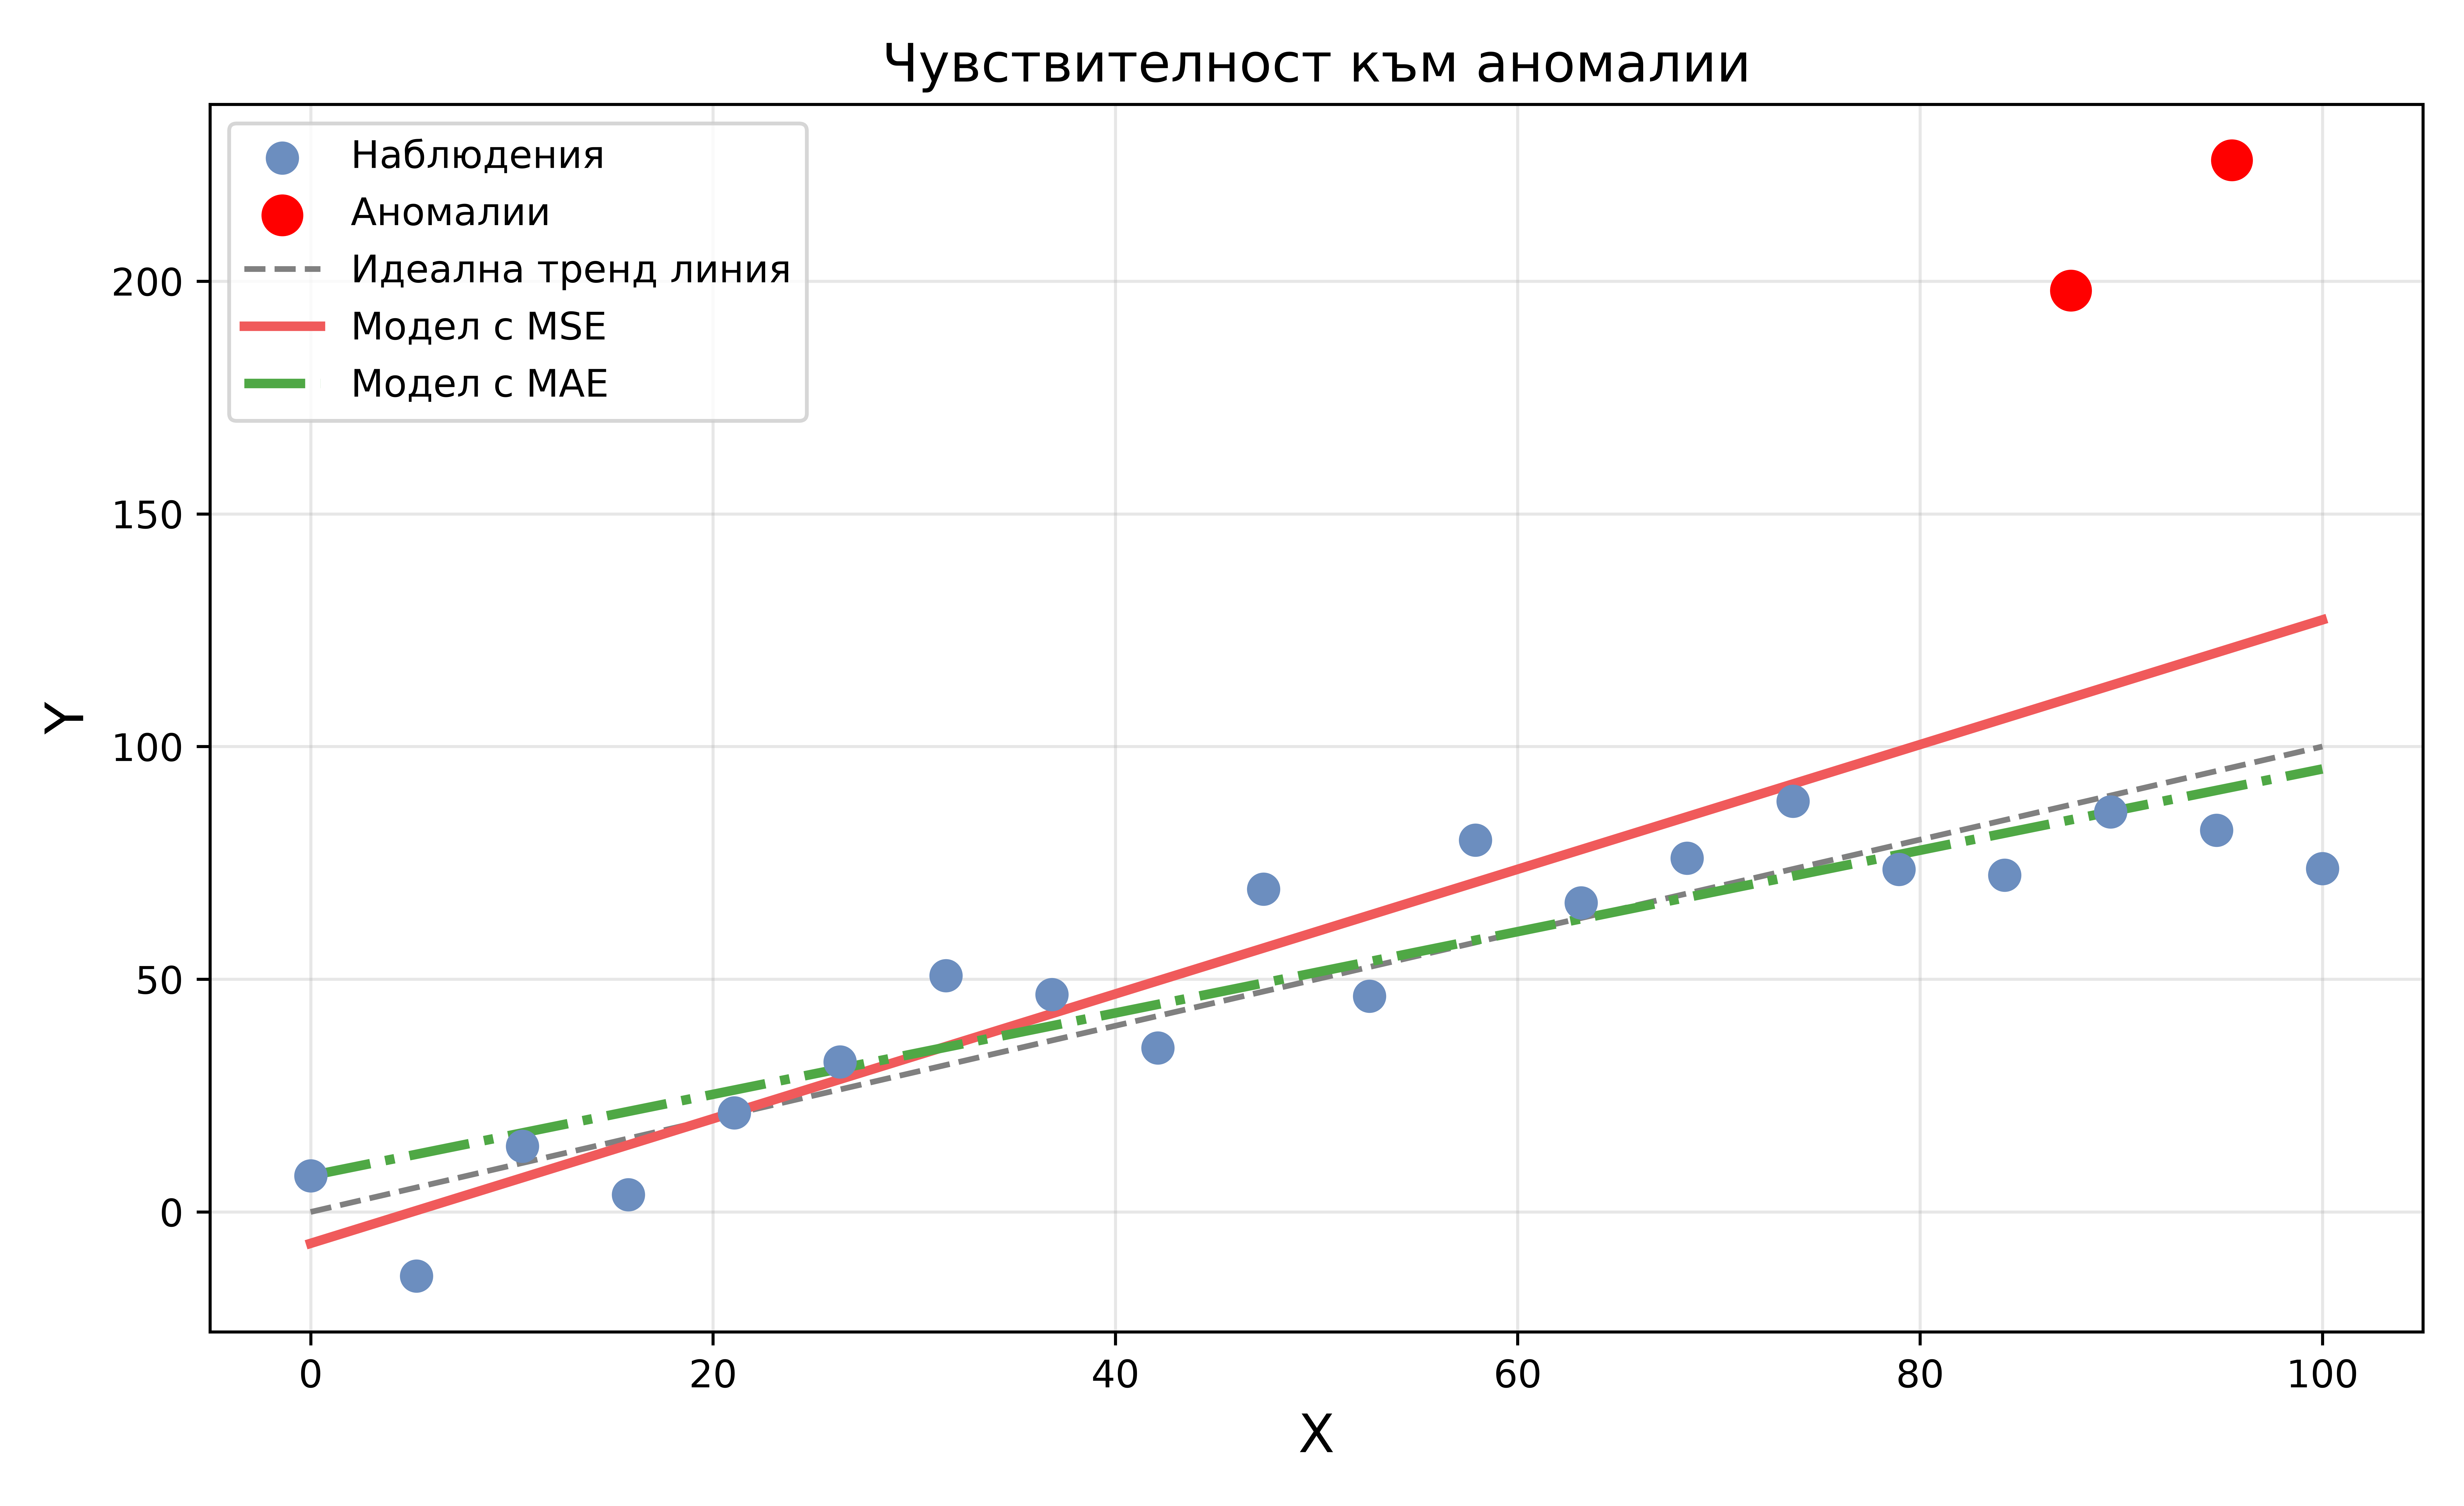
\includegraphics[width=0.55\paperwidth]{images/reg_metrics_sensitivity_to_outliers.png}
      };
    \end{tikzpicture}
  \end{columns}
\end{frame}

% --------------------------------------------------------------------------------

\begin{frame}
  \begin{columns}[T, onlytextwidth]
    \begin{column}{0.6\textwidth}
      \begin{itemize}
        \item Как оценяваме грешката на модела?
          \begin{itemize}
            \item \textbf{Избор на метрика}
            \item Метод на валидация
          \end{itemize}

          \vspace{0.1cm}

        \item Метрики за класификация
      \end{itemize}

      \hspace*{-2cm}
      \begin{minipage}{\linewidth}
        \small
        \begin{align*}
          \text{Accuracy} &= \frac{\text{TP} + \text{TN}}{\text{TP} + \text{FP} + \text{TN} + \text{FN}} \\[8pt]
          \text{Precision} &= \frac{\text{TP}}{\text{TP} + \text{FP}} \\[8pt]
          \text{Sensitivity (Recall)} &= \frac{\text{TP}}{\text{TP} + \text{FN}} \\[8pt]
          \text{Specificity} &= \frac{\text{TN}}{\text{TN} + \text{FP}} \\[8pt]
          \text{NPV} &= \frac{\text{TN}}{\text{TN} + \text{FN}} \\[8pt]
          \text{AUC} &= \int_0^1 \text{TPR}(t) \, d(\text{FPR}(t))
        \end{align*}
      \end{minipage}
    \end{column}
    
    \begin{tikzpicture}[remember picture, overlay]
      \node[anchor=east] at ([xshift=-1.3cm, yshift=2.3cm]current page.east) {
        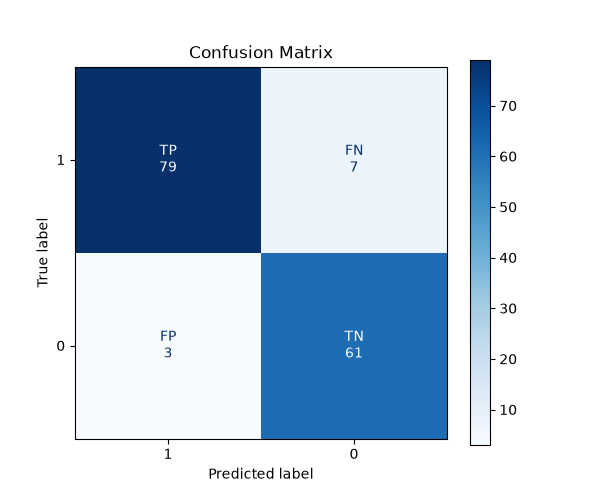
\includegraphics[width=0.35\paperwidth]{images/confusion_matrix_binary.png}
      };
      \node[anchor=east] at ([xshift=-2cm, yshift=-2.1cm]current page.east) {
        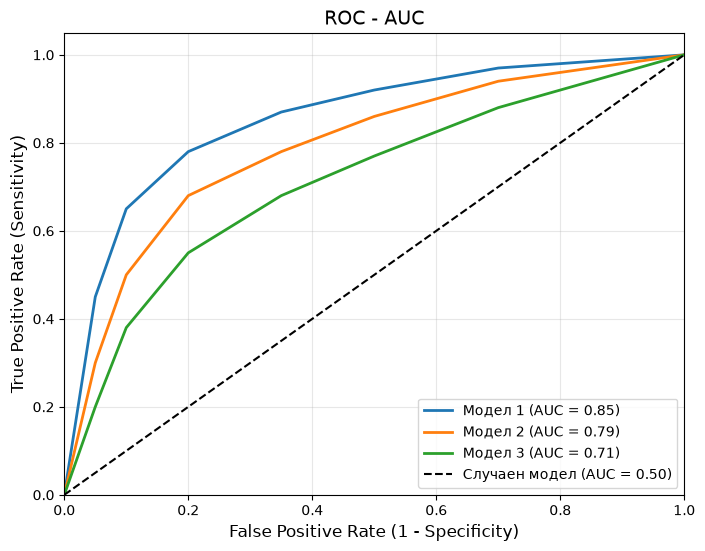
\includegraphics[width=0.3\paperwidth]{images/auc_metric.png}
      };
    \end{tikzpicture}
  \end{columns}
\end{frame}

% --------------------------------------------------------------------------------

\begin{frame}
  \begin{columns}[T, onlytextwidth]
    \begin{column}{0.6\textwidth}
      \begin{itemize}
        \item Как оценяваме грешката на модела?
          \begin{itemize}
            \item \textbf{Избор на метрика}
            \item Метод на валидация
          \end{itemize}
            \vspace{0.1cm}
        \item Метрики за класификация и проблем с дисбаланс на класовете\\
        \vspace{0.5ex}
        {\small\itshape\color{gray} (напр. прогнозиране на рядка болест с честота 0.5\%)}
      \end{itemize}

      \hspace*{-1.65cm}
      \begin{minipage}{\linewidth}
        \small
        \begin{align*}
          {\color{red}\text{Accuracy}} &= \frac{\text{TP} + \text{TN}}{\text{TP} + \text{FP} + \text{TN} + \text{FN}} = 99.5\% \\[6pt]
          {\color{green}\text{Precision}} &= \frac{\text{TP}}{\text{TP} + \text{FP}} = 0\% \ (\text{undefined}) \\[6pt]
          {\color{green}\text{Sensitivity (Recall)}} &= \frac{\text{TP}}{\text{TP} + \text{FN}} = 0\% \\[6pt]
          {\color{orange}\text{Specificity}} &= \frac{\text{TN}}{\text{TN} + \text{FP}} = 100\%\\[6pt]
          {\color{orange}\text{NPV}} &= \frac{\text{TN}}{\text{TN} + \text{FN}} = 99.5\% 
        \end{align*}
      \end{minipage}
    \end{column}

    \begin{column}[T, onlytextwidth]{0.4\textwidth}
      \begin{block}{\small Фокус върху позитивния клас}
        \scriptsize
        \textbf{Precision} и \textbf{Sensitivity} не се влияят от дисбаланса, когато позитивния клас е малцинствен.
      \end{block}

      \begin{block}{\small Фокус върху негативния клас}
        \scriptsize
        \textbf{Specificity} и \textbf{NPV} не се влияят от дисбаланса, когато негативния клас е малцинствен.
      \end{block}

      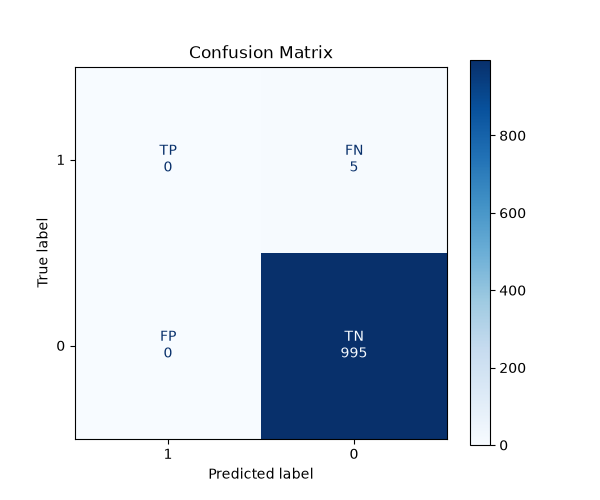
\includegraphics[width=0.35\paperwidth]{images/confusion_matrix_imbalance.png}
    \end{column}
  \end{columns}
\end{frame}

% --------------------------------------------------------------------------------

\begin{frame}
  \begin{columns}[T, onlytextwidth]
    \begin{column}{0.5\textwidth}
      \begin{itemize}
        \item Как оценяваме грешката на модела?
          \begin{itemize}
            \item \textbf{Избор на метрика}
            \item Метод на валидация
          \end{itemize}
        \item Метрики за многокласова класификация:\\
        \vspace{0.5ex}
        {\small\itshape\color{gray} (принцип 1 срещу всички останали)}
      \end{itemize}

      \hspace*{1cm}
      \begin{align*}
          \text{Macro-average} &= \frac{1}{\text{K}}\sum_{i}^{\text{K}} \text{Metric}_i, \quad \text{Metric}_i = \text{метрика за клас } i \\ 
          \text{Weighted-average} &= \frac{\sum_{i}^{\text{K}} w_i \cdot \text{Metric}_i}{\sum_{i}^{\text{K}} w_i}, \quad w_i = \text{честота на клас } i \\ 
          \text{Micro-average} &= \frac{\sum_{i}^{\text{K}} \text{TP}_i}{\sum_{i}^{\text{K}} (\text{TP}_i + \text{FP}_i + \text{FN}_i)}
      \end{align*}
    \end{column}

    \begin{tikzpicture}[remember picture, overlay]
      \node[anchor=east] at ([xshift=-0.8cm, yshift=2.3cm]current page.east) {
        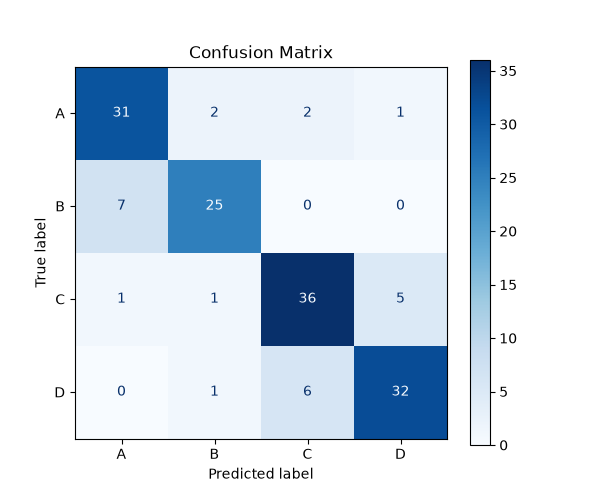
\includegraphics[width=0.35\paperwidth]{images/confusion_matrix_multi_class.png}
      };
    \end{tikzpicture}
  \end{columns}
\end{frame}

% --------------------------------------------------------------------------------

\subsection{Валидация}

% --------------------------------------------------------------------------------

\begin{frame}
  \begin{itemize}
    \item Как оценяваме грешката на модела?
      \begin{itemize}
        \item Избор на метрика
        \item \textbf{Метод на валидация}
      \end{itemize}
    \item Преобучение (Overfitting)
    \vspace{0.5ex}
  \end{itemize}

  \centering
  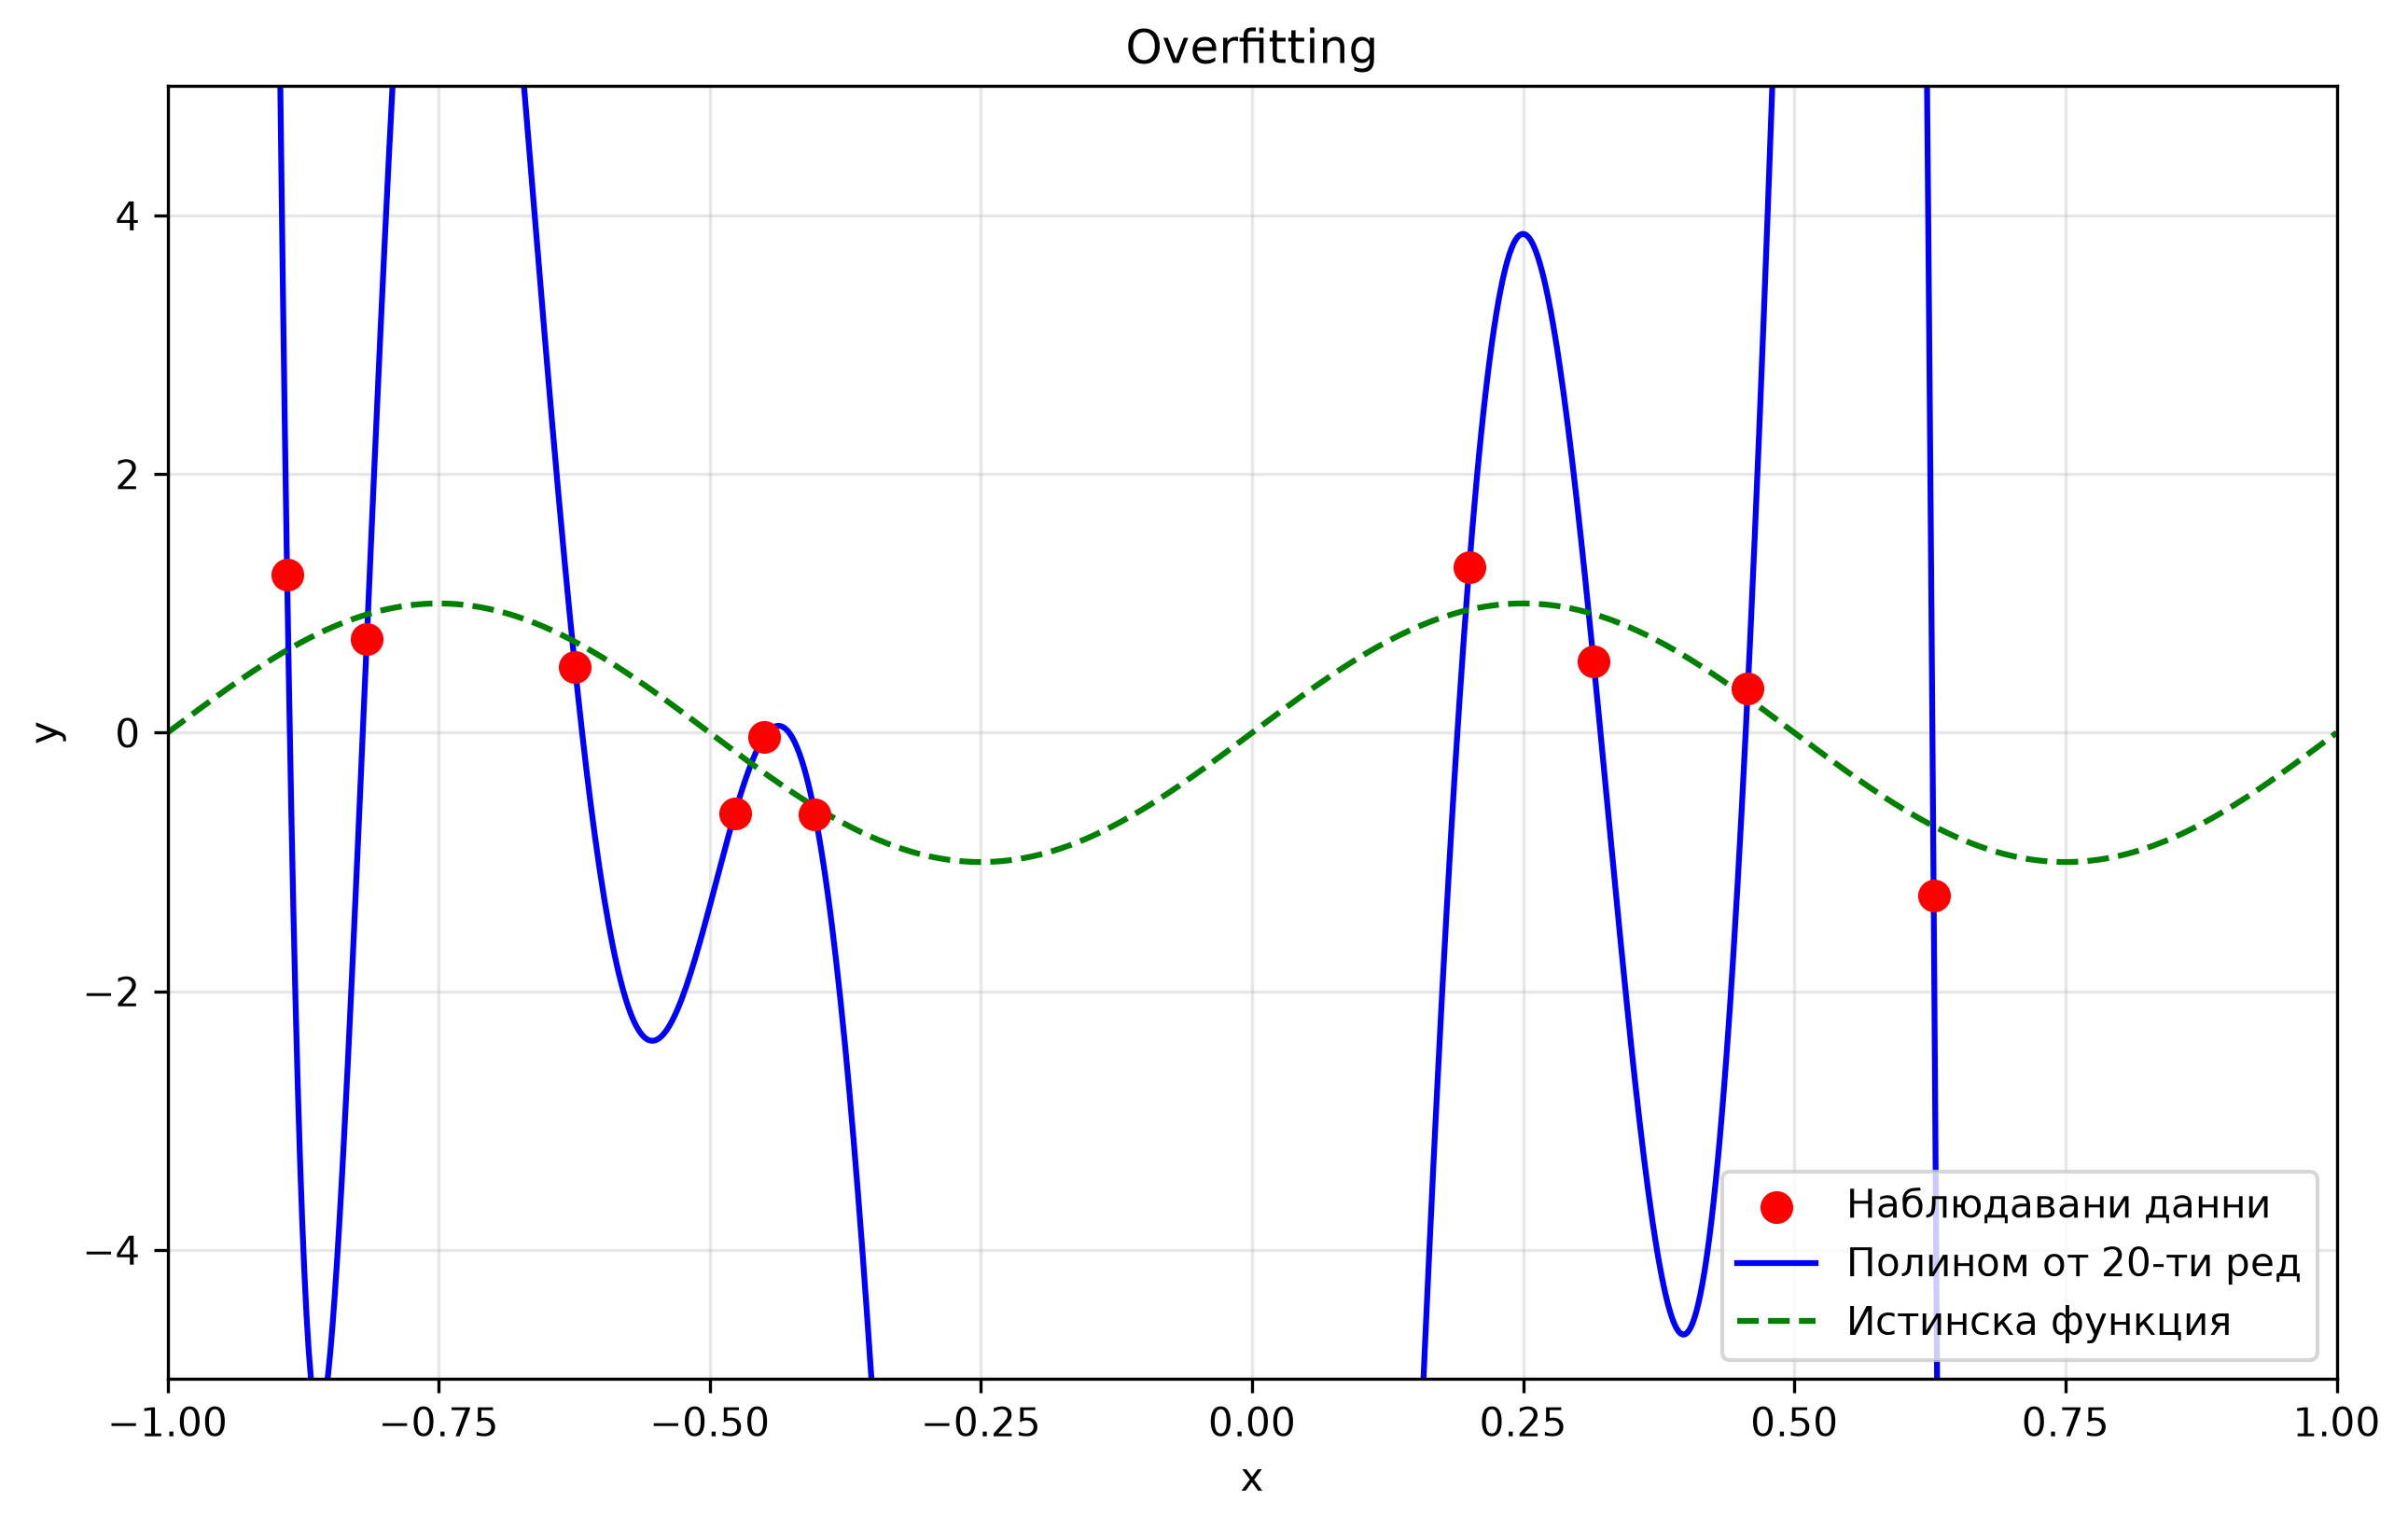
\includegraphics[width=0.45\textwidth]{images/overfitting_1.png}
  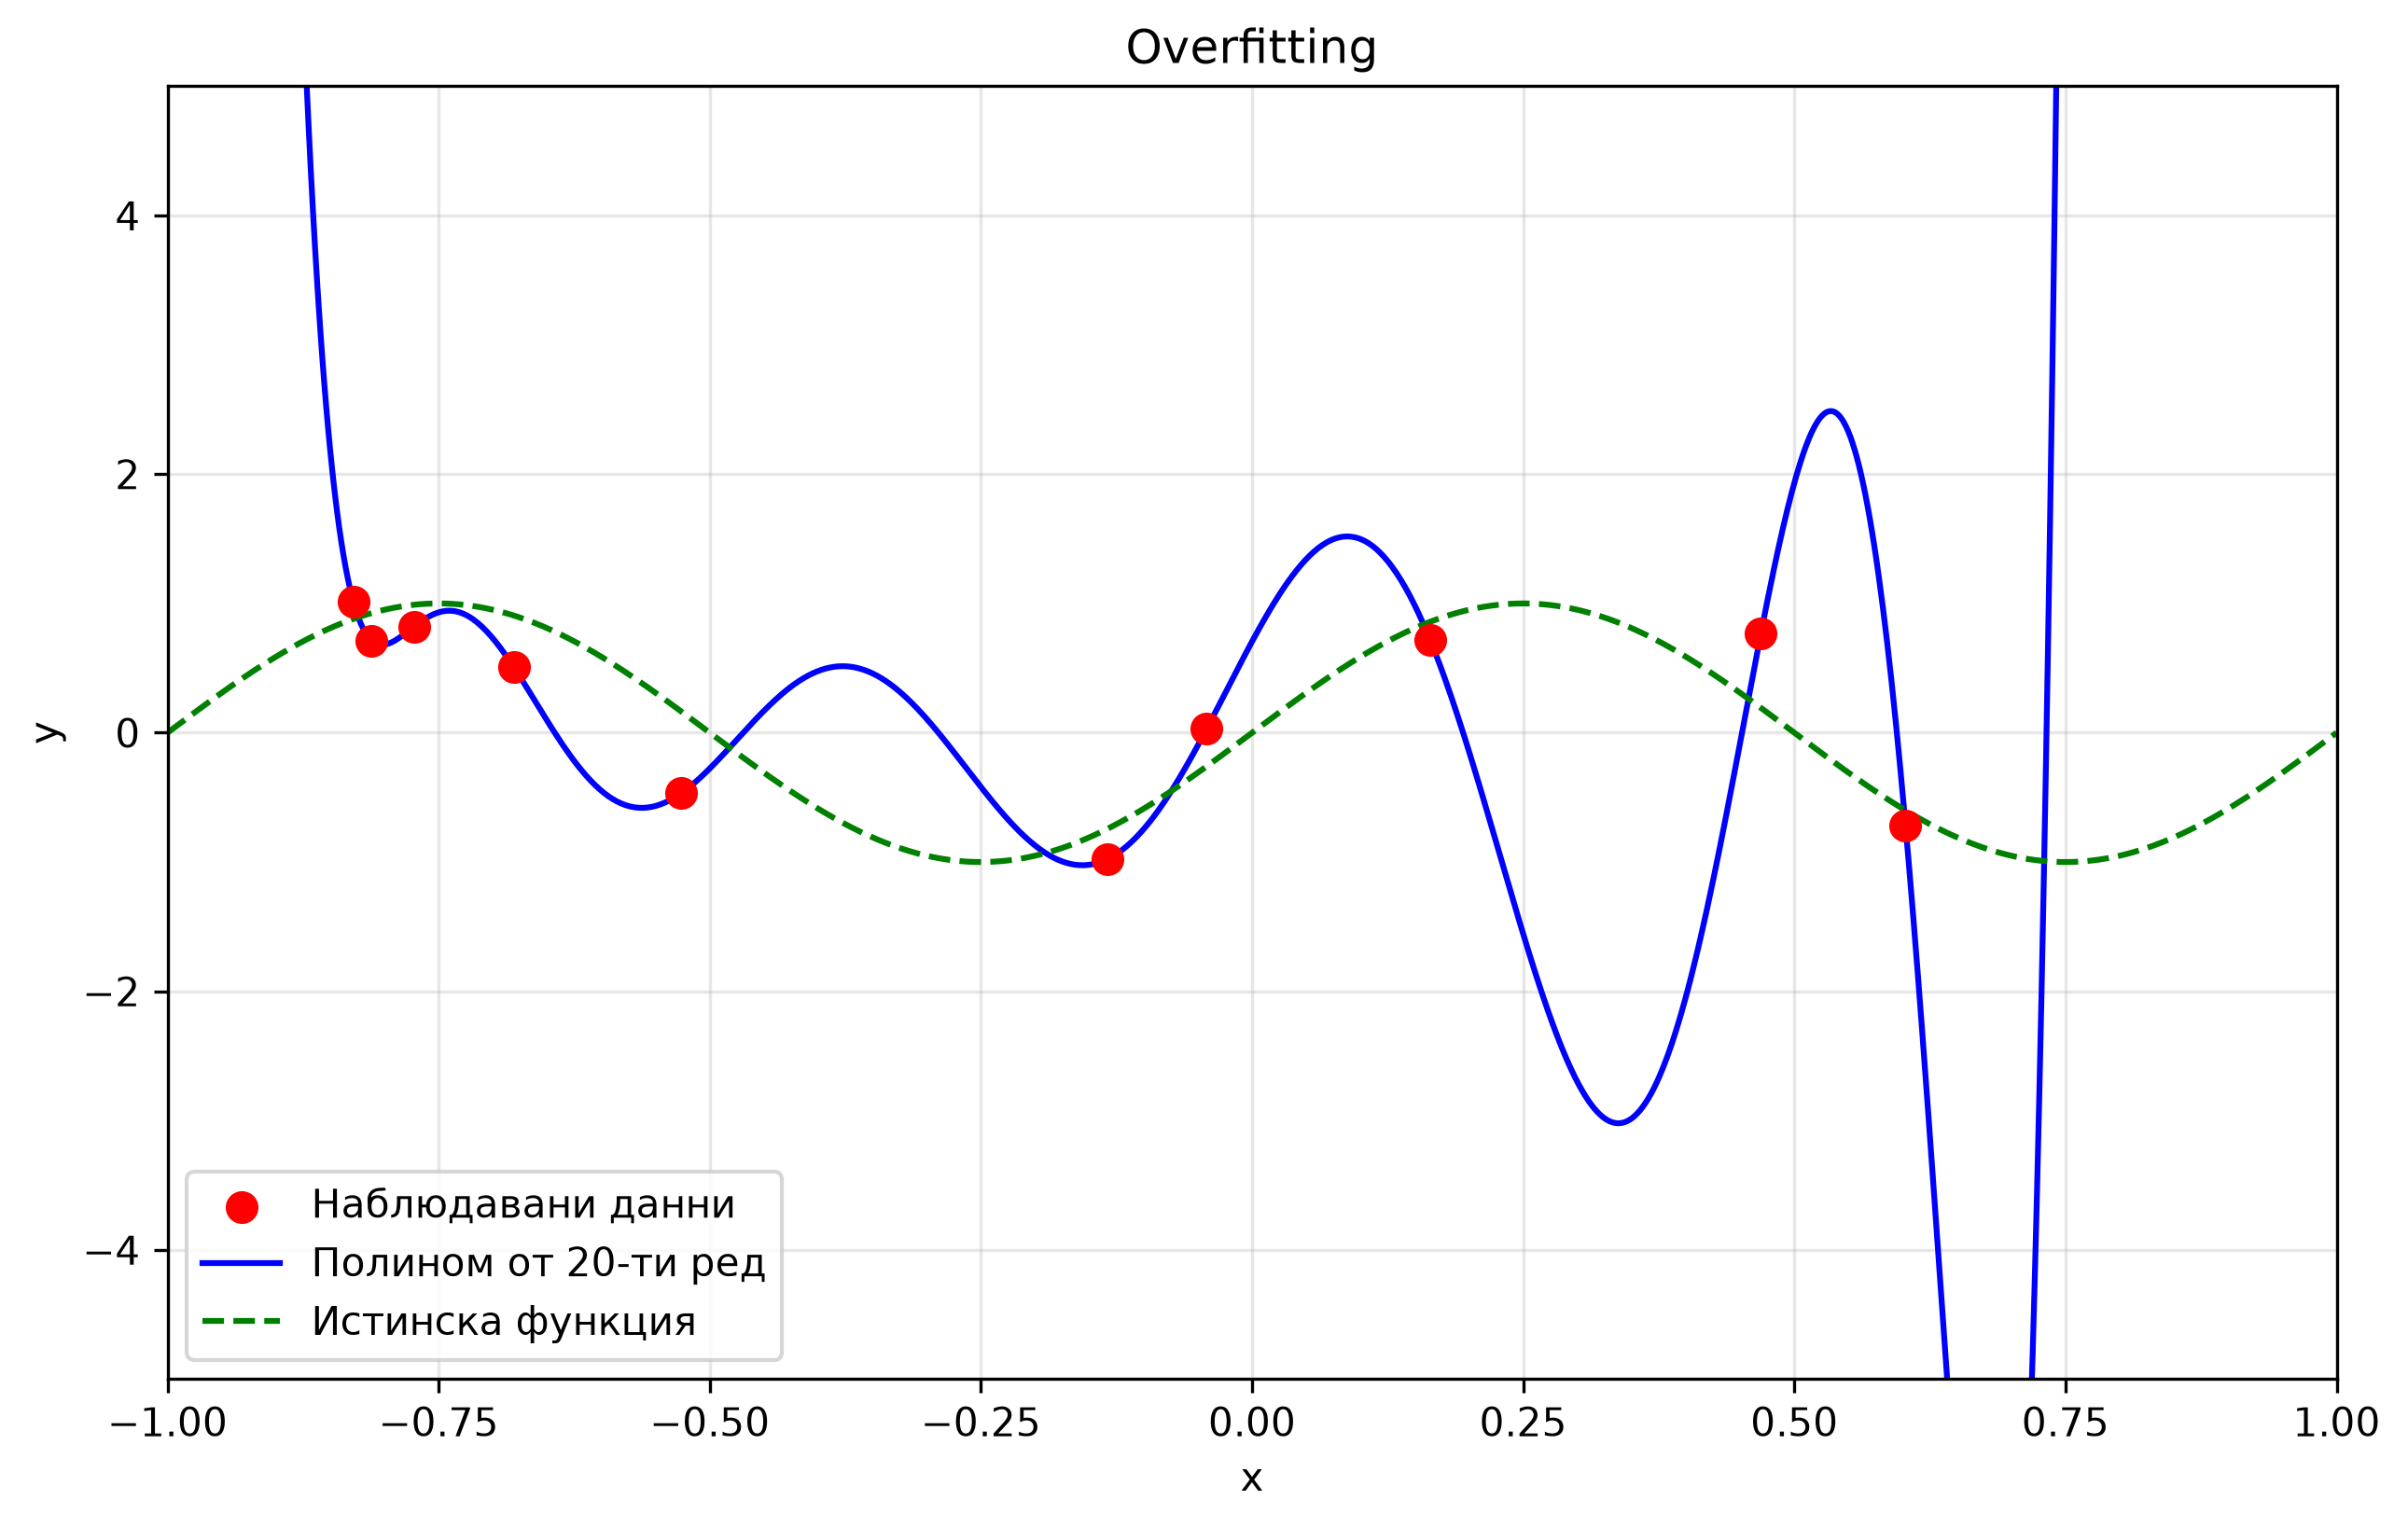
\includegraphics[width=0.45\textwidth]{images/overfitting_2.png}

  \begin{itemize}
    \item Очакваната грешка $\mathbb{E}[(\mathbf{Y} - \mathbf{\hat{Y}})^2]$ се доминира от вариацията $\text{Var}[\mathbf{\hat{f}}]$. \secref{subsection:систематична_грешка_и_вариация}
  \end{itemize}
\end{frame}

% --------------------------------------------------------------------------------

\begin{frame}
  \begin{itemize}
    \item Как оценяваме грешката на модела?
      \begin{itemize}
        \item Избор на метрика
        \item \textbf{Метод на валидация}
      \end{itemize}
    \item Недообучение (Underfitting)
    \vspace{0.5ex}
  \end{itemize}

  \centering
  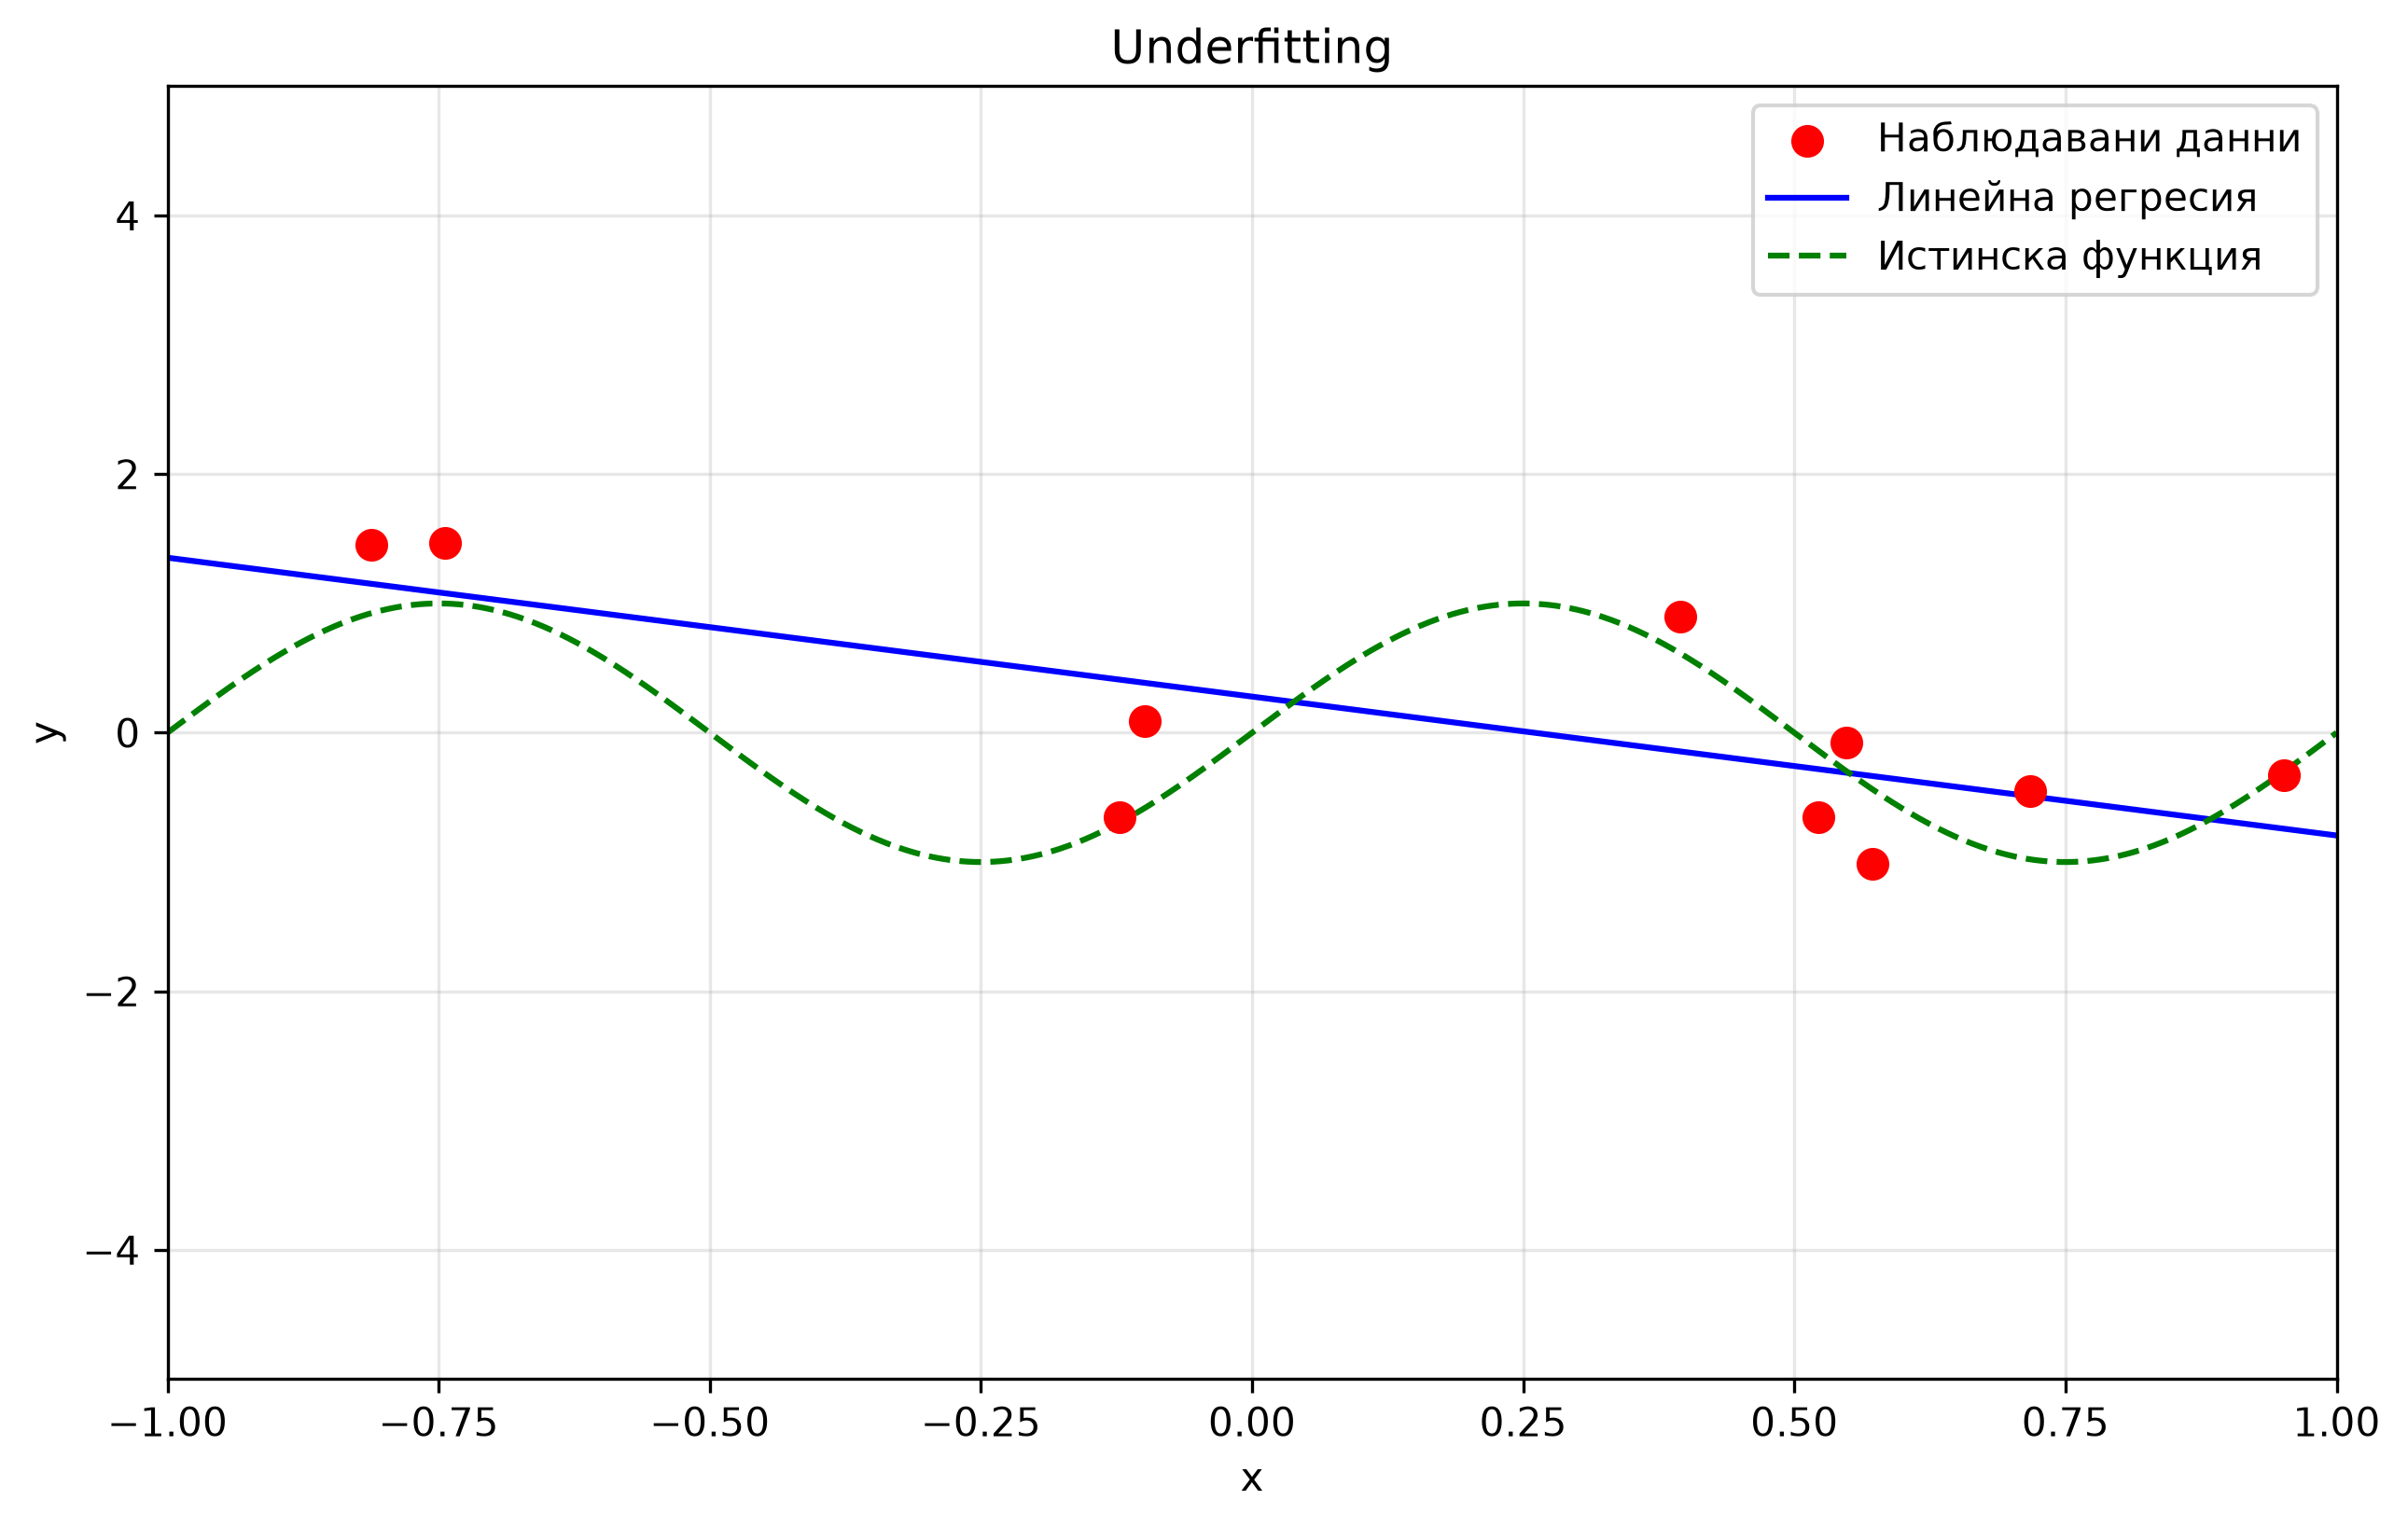
\includegraphics[width=0.45\textwidth]{images/underfitting_1.png}
  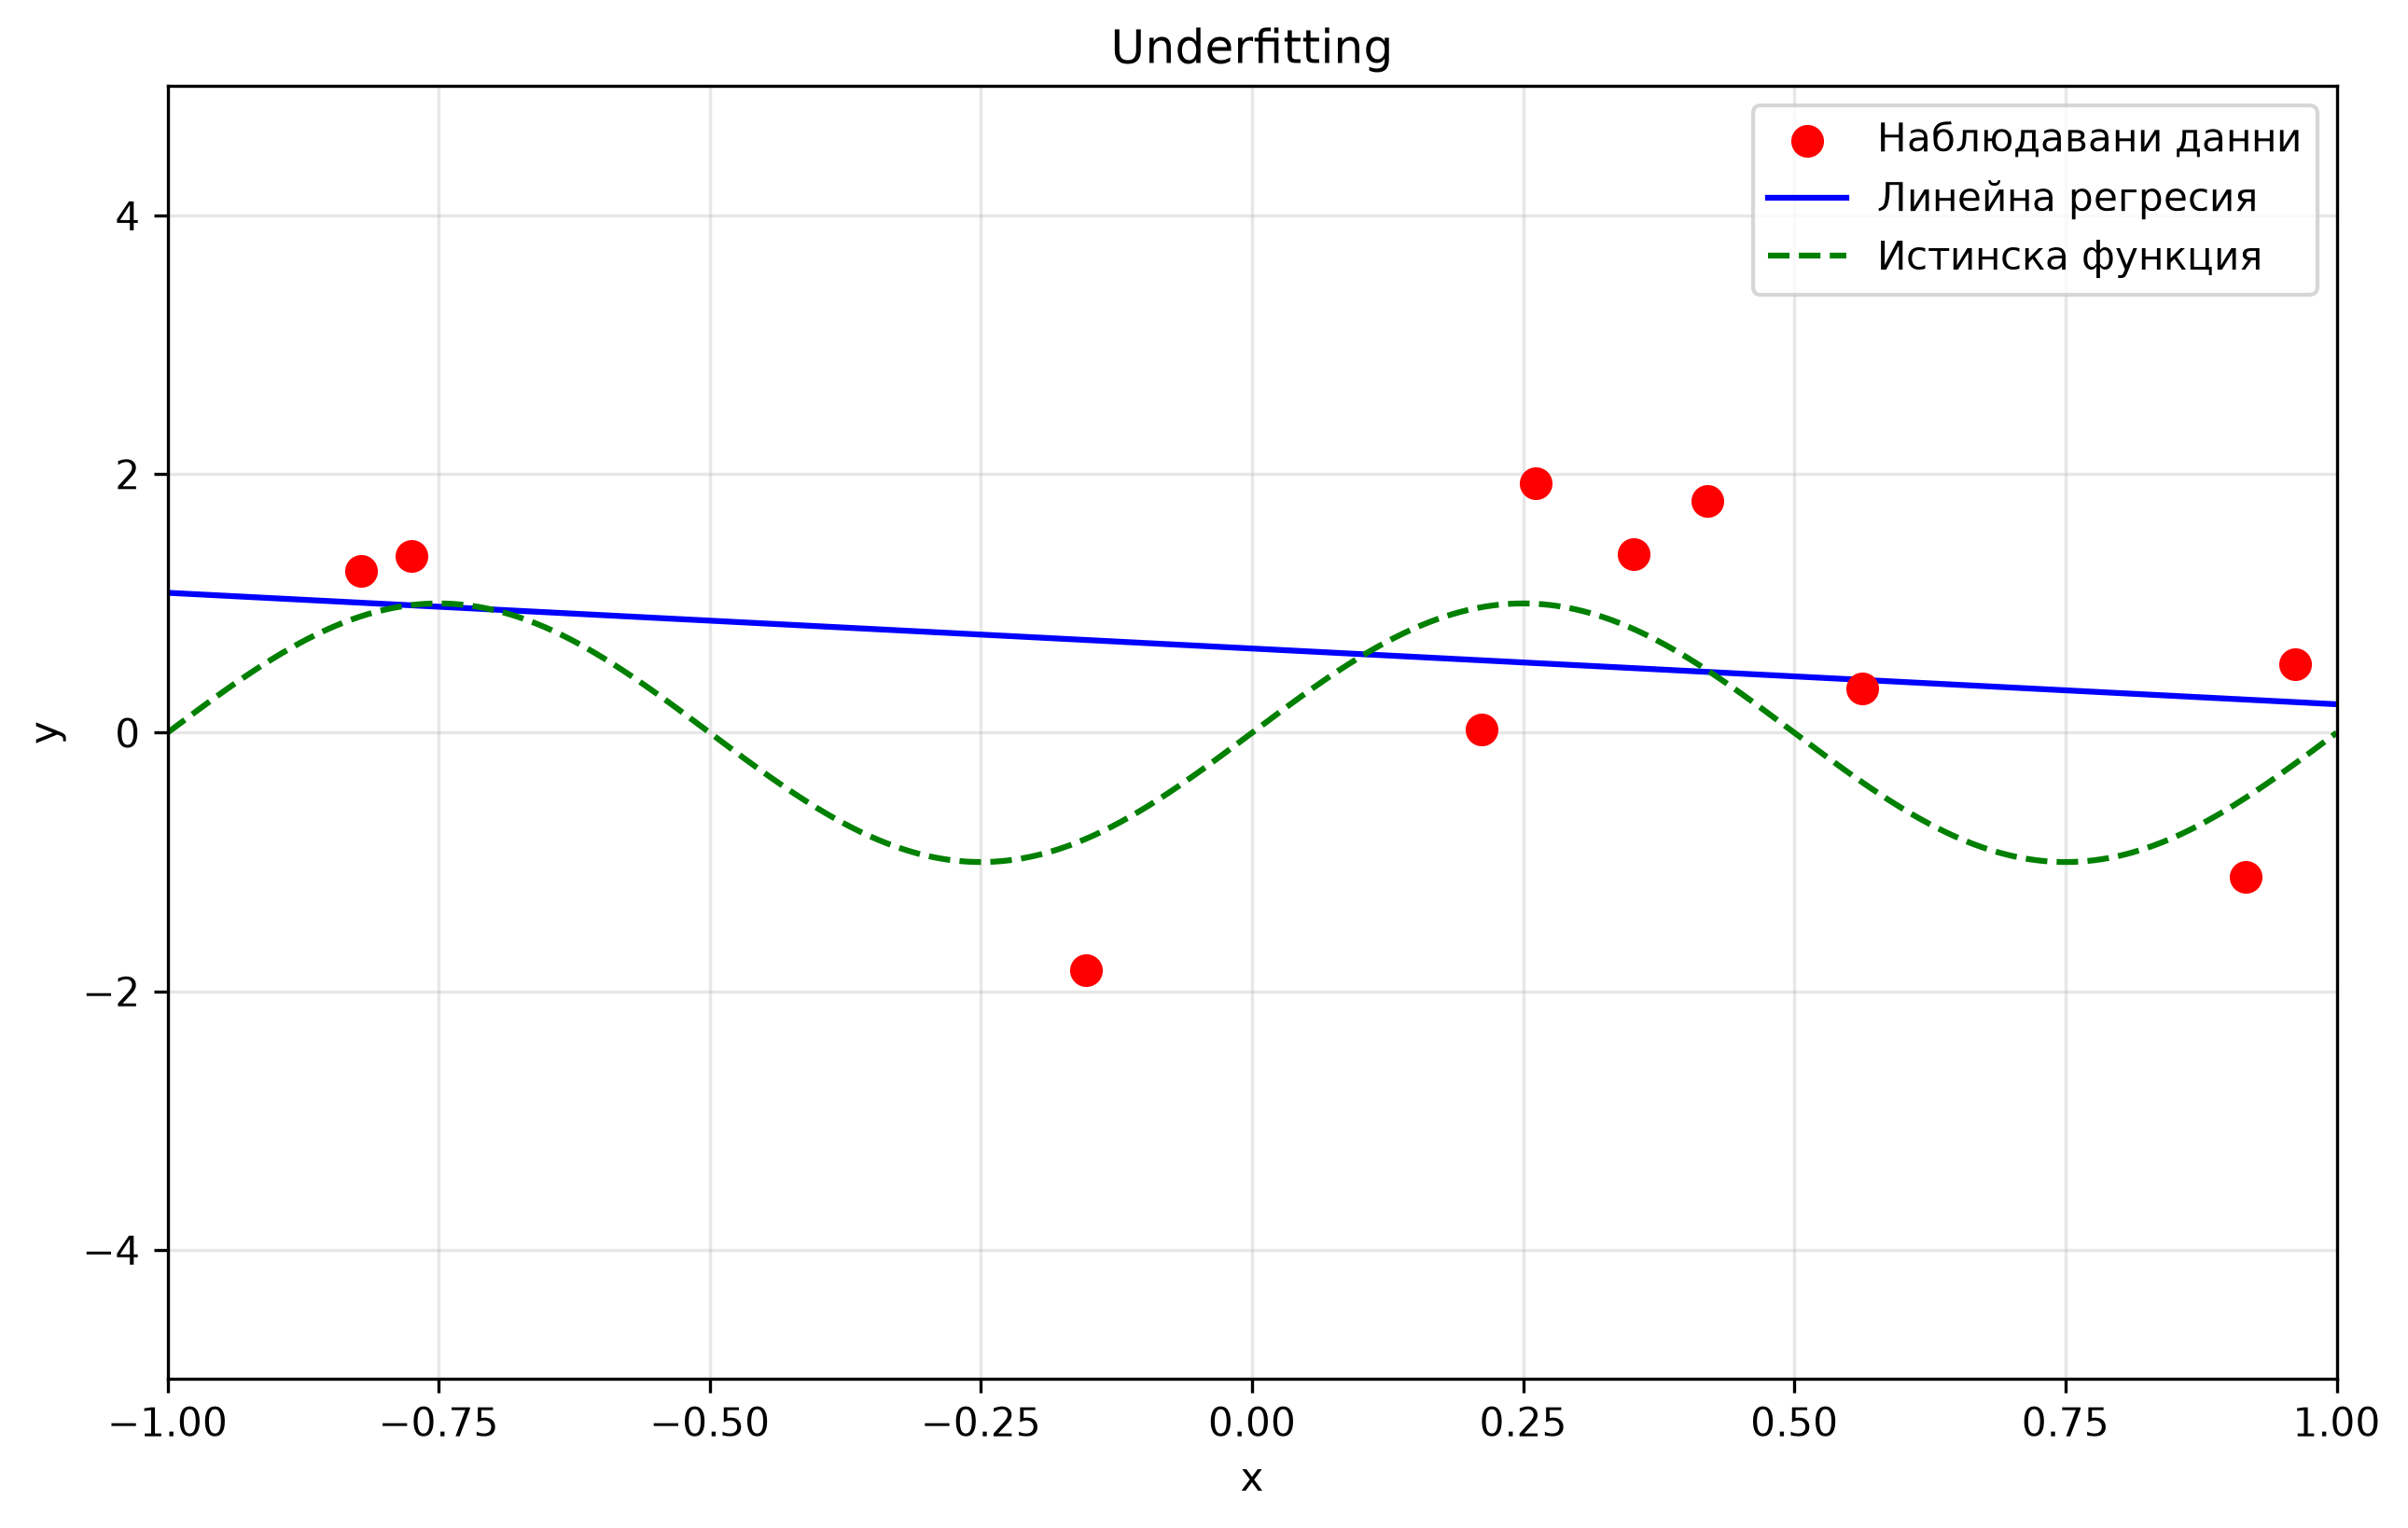
\includegraphics[width=0.45\textwidth]{images/underfitting_2.png}
  
  \begin{itemize}
    \item Очакваната грешка $\mathbb{E}[(\mathbf{Y} - \mathbf{\hat{Y}})^2]$ се доминира от систематичната грешка $(f - \mathbb{E}[\hat{f}])^2$. \secref{subsection:систематична_грешка_и_вариация}
  \end{itemize}
\end{frame}

% --------------------------------------------------------------------------------

\begin{frame}
  \begin{itemize}
    \item Как оценяваме грешката на модела?
      \begin{itemize}
        \item Избор на метрика
        \item \textbf{Метод на валидация}
      \end{itemize}
    \item {\color{red}Нужен е метод, който да оцени грешката правилно имайки предвид преобучението и недообучението!!!}
    \begin{itemize}
      \item Висока грешка при недообучение (Underfitting)
      \item Висока грешка при преобучение (Overfitting)
    \end{itemize}

    \centering
    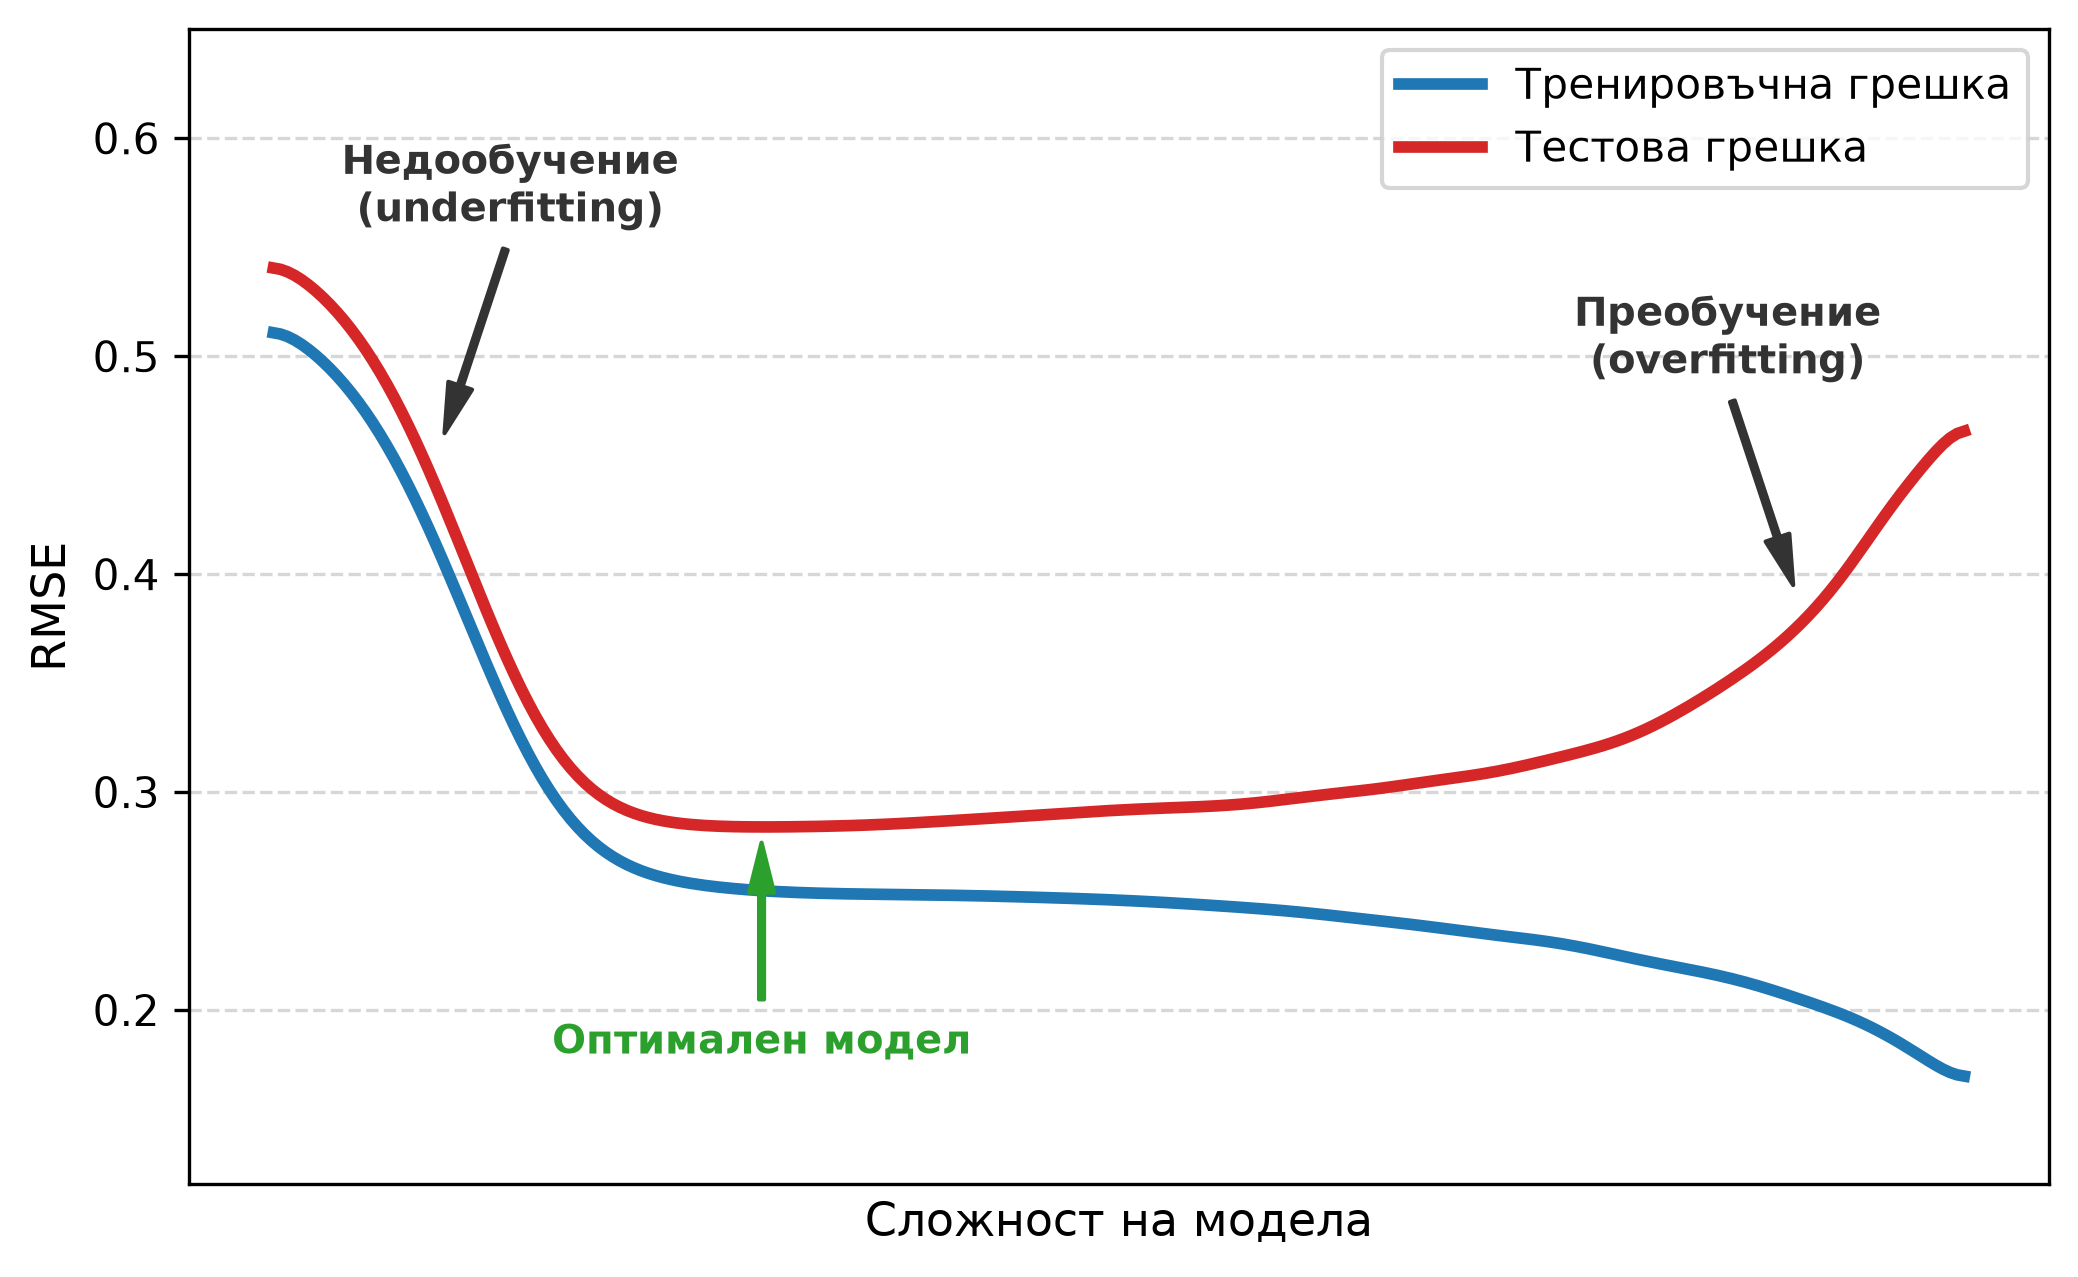
\includegraphics[width=0.5\textwidth]{images/train_test_scores_model_complexity.png}
  \end{itemize}
\end{frame}

% --------------------------------------------------------------------------------

\begin{frame}
  \begin{itemize}
    \item Как оценяваме грешката на модела?
      \begin{itemize}
        \item Избор на метрика
        \item \textbf{Метод на валидация}
      \end{itemize}
    \item {\color{red}Нужен е метод, който да оцени грешката правилно имайки предвид преобучението и недообучението!!!}
    \begin{itemize}
      \item Тренировъчната оценка подценява истинската грешка при преобучение (Overfitting)
      \item Тестовата оценка дава по-точна представа за истинската грешка
    \end{itemize}

    \centering
    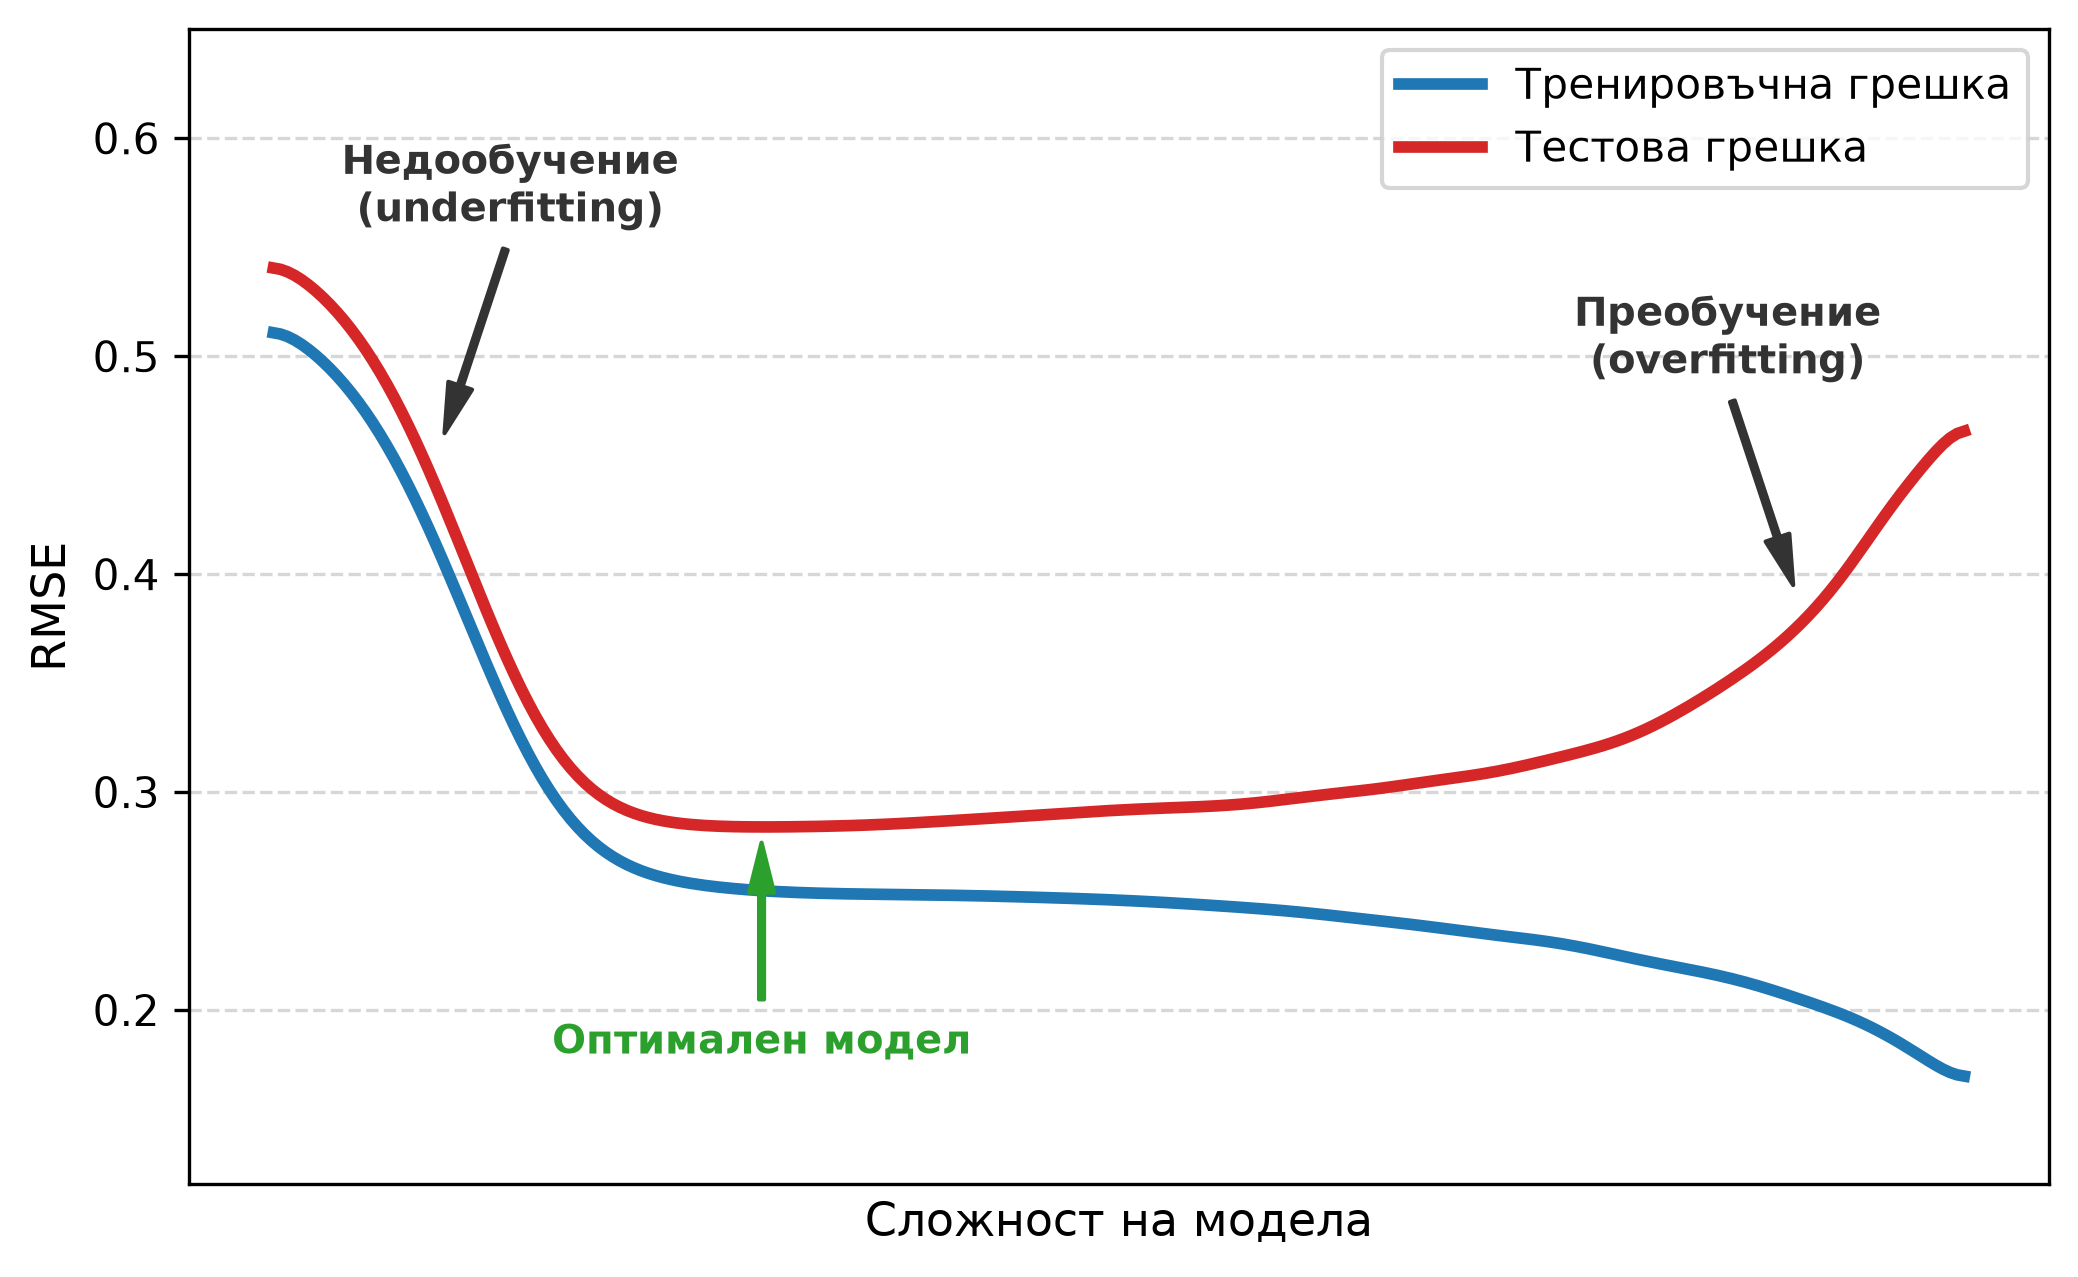
\includegraphics[width=0.5\textwidth]{images/train_test_scores_model_complexity.png}
  \end{itemize}
\end{frame}

% --------------------------------------------------------------------------------

\subsubsection{Тренировъчна и тестова оценка}

% --------------------------------------------------------------------------------

\begin{frame}
  \begin{itemize}
    \item Как оценяваме грешката на модела?
      \begin{itemize}
        \item Избор на метрика
        \item \textbf{Метод на валидация}
      \end{itemize}
    \item Разделяне на тренировъчни и тестови данни (train-test split)\\
    {\small\itshape\color{gray} Тренираме на тренировъчните данни и оценяваме на тестовите данни.}
    
    \vspace{1ex}

    \centering
    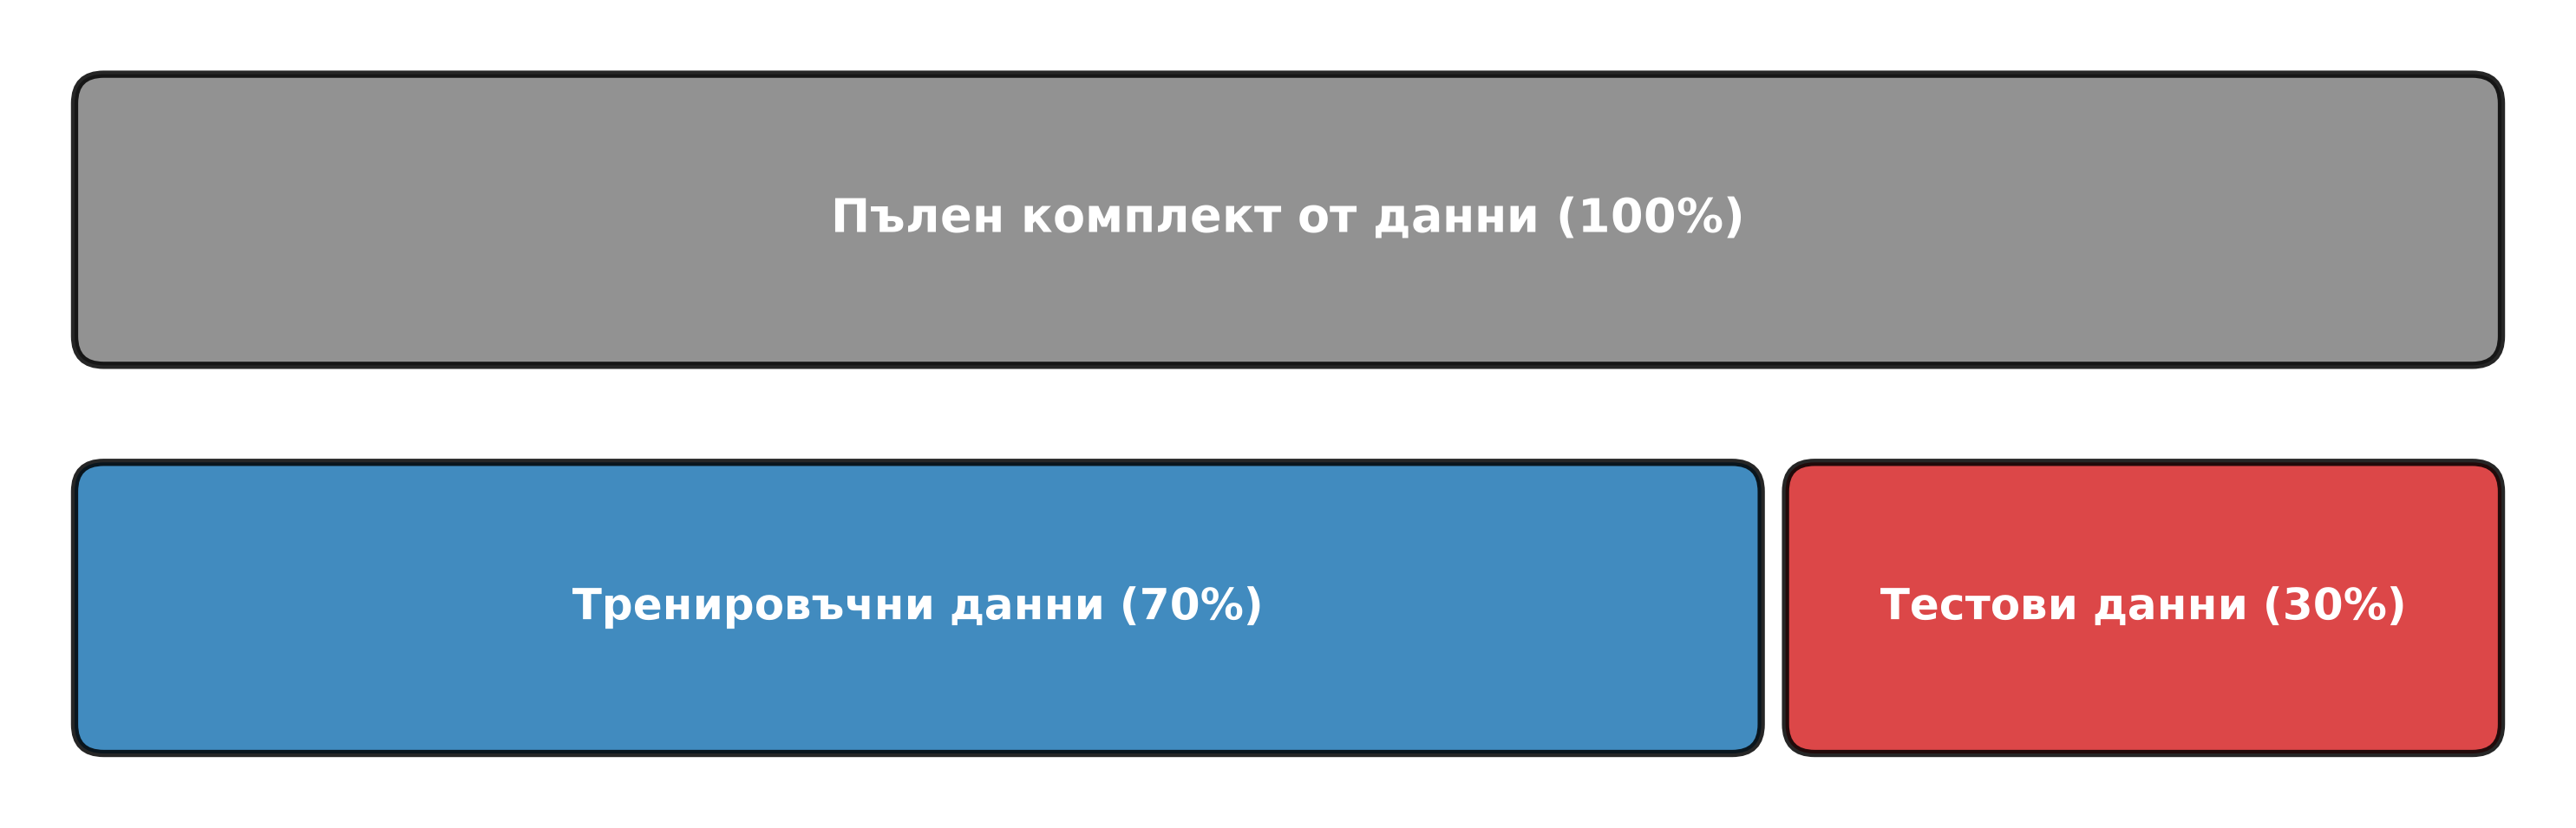
\includegraphics[width=0.5\textwidth]{images/train_test_split.png}
  \end{itemize}
\end{frame}

% --------------------------------------------------------------------------------

\subsubsection{Кръстосана валидация}

% --------------------------------------------------------------------------------

\begin{frame}
  \begin{itemize}
    \item Как оценяваме грешката на модела?
      \begin{itemize}
        \item Избор на метрика
        \item \textbf{Метод на валидация}
      \end{itemize}
    \item k-кратна кръстосана валидация (k-fold cross-validation)\\
    {\small\itshape\color{gray} Разделяме данните неколкократно, тренираме на част от тях и тестваме на останалите, като повтаряме процеса.}
    
    \vspace{1ex}

    \centering
    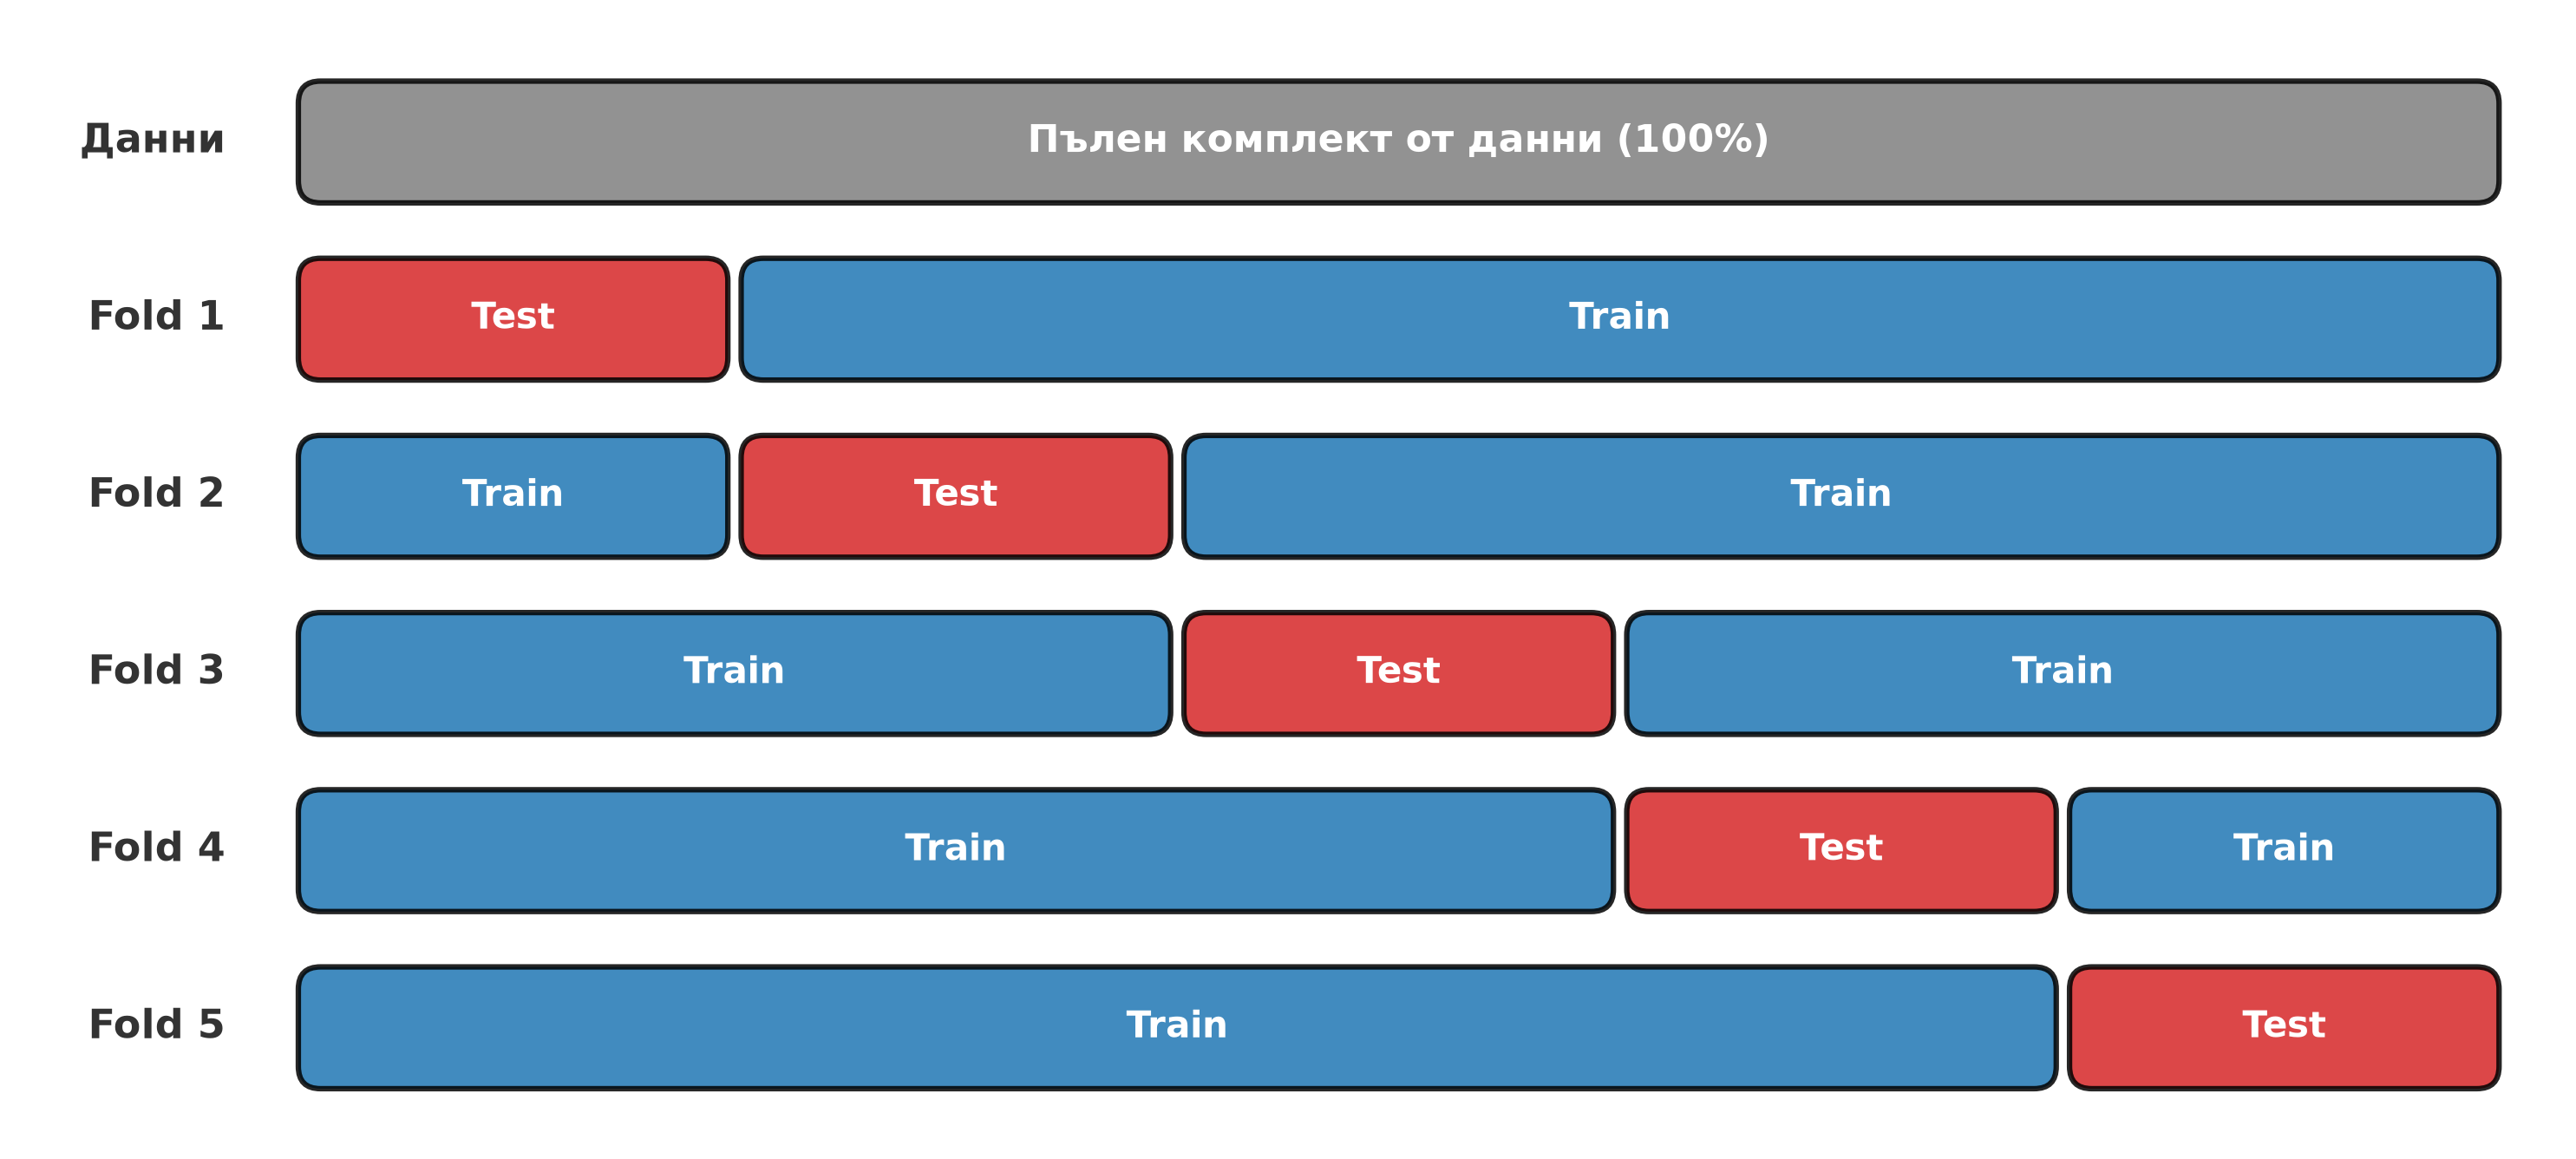
\includegraphics[width=0.7\textwidth]{images/5fold_cross_validation.png}
  \end{itemize}
\end{frame}

% --------------------------------------------------------------------------------

\begin{frame}
  \begin{itemize}
    \item Как оценяваме грешката на модела?
      \begin{itemize}
        \item Избор на метрика
        \item \textbf{Метод на валидация}
      \end{itemize}
    \item k-кратна кръстосана валидация (k-fold cross-validation)\\
    {\small\itshape\color{gray} Разделяме данните неколкократно, тренираме на част от тях и тестваме на останалите, като повтаряме процеса.}
    
    \vspace{1ex}

    \centering
    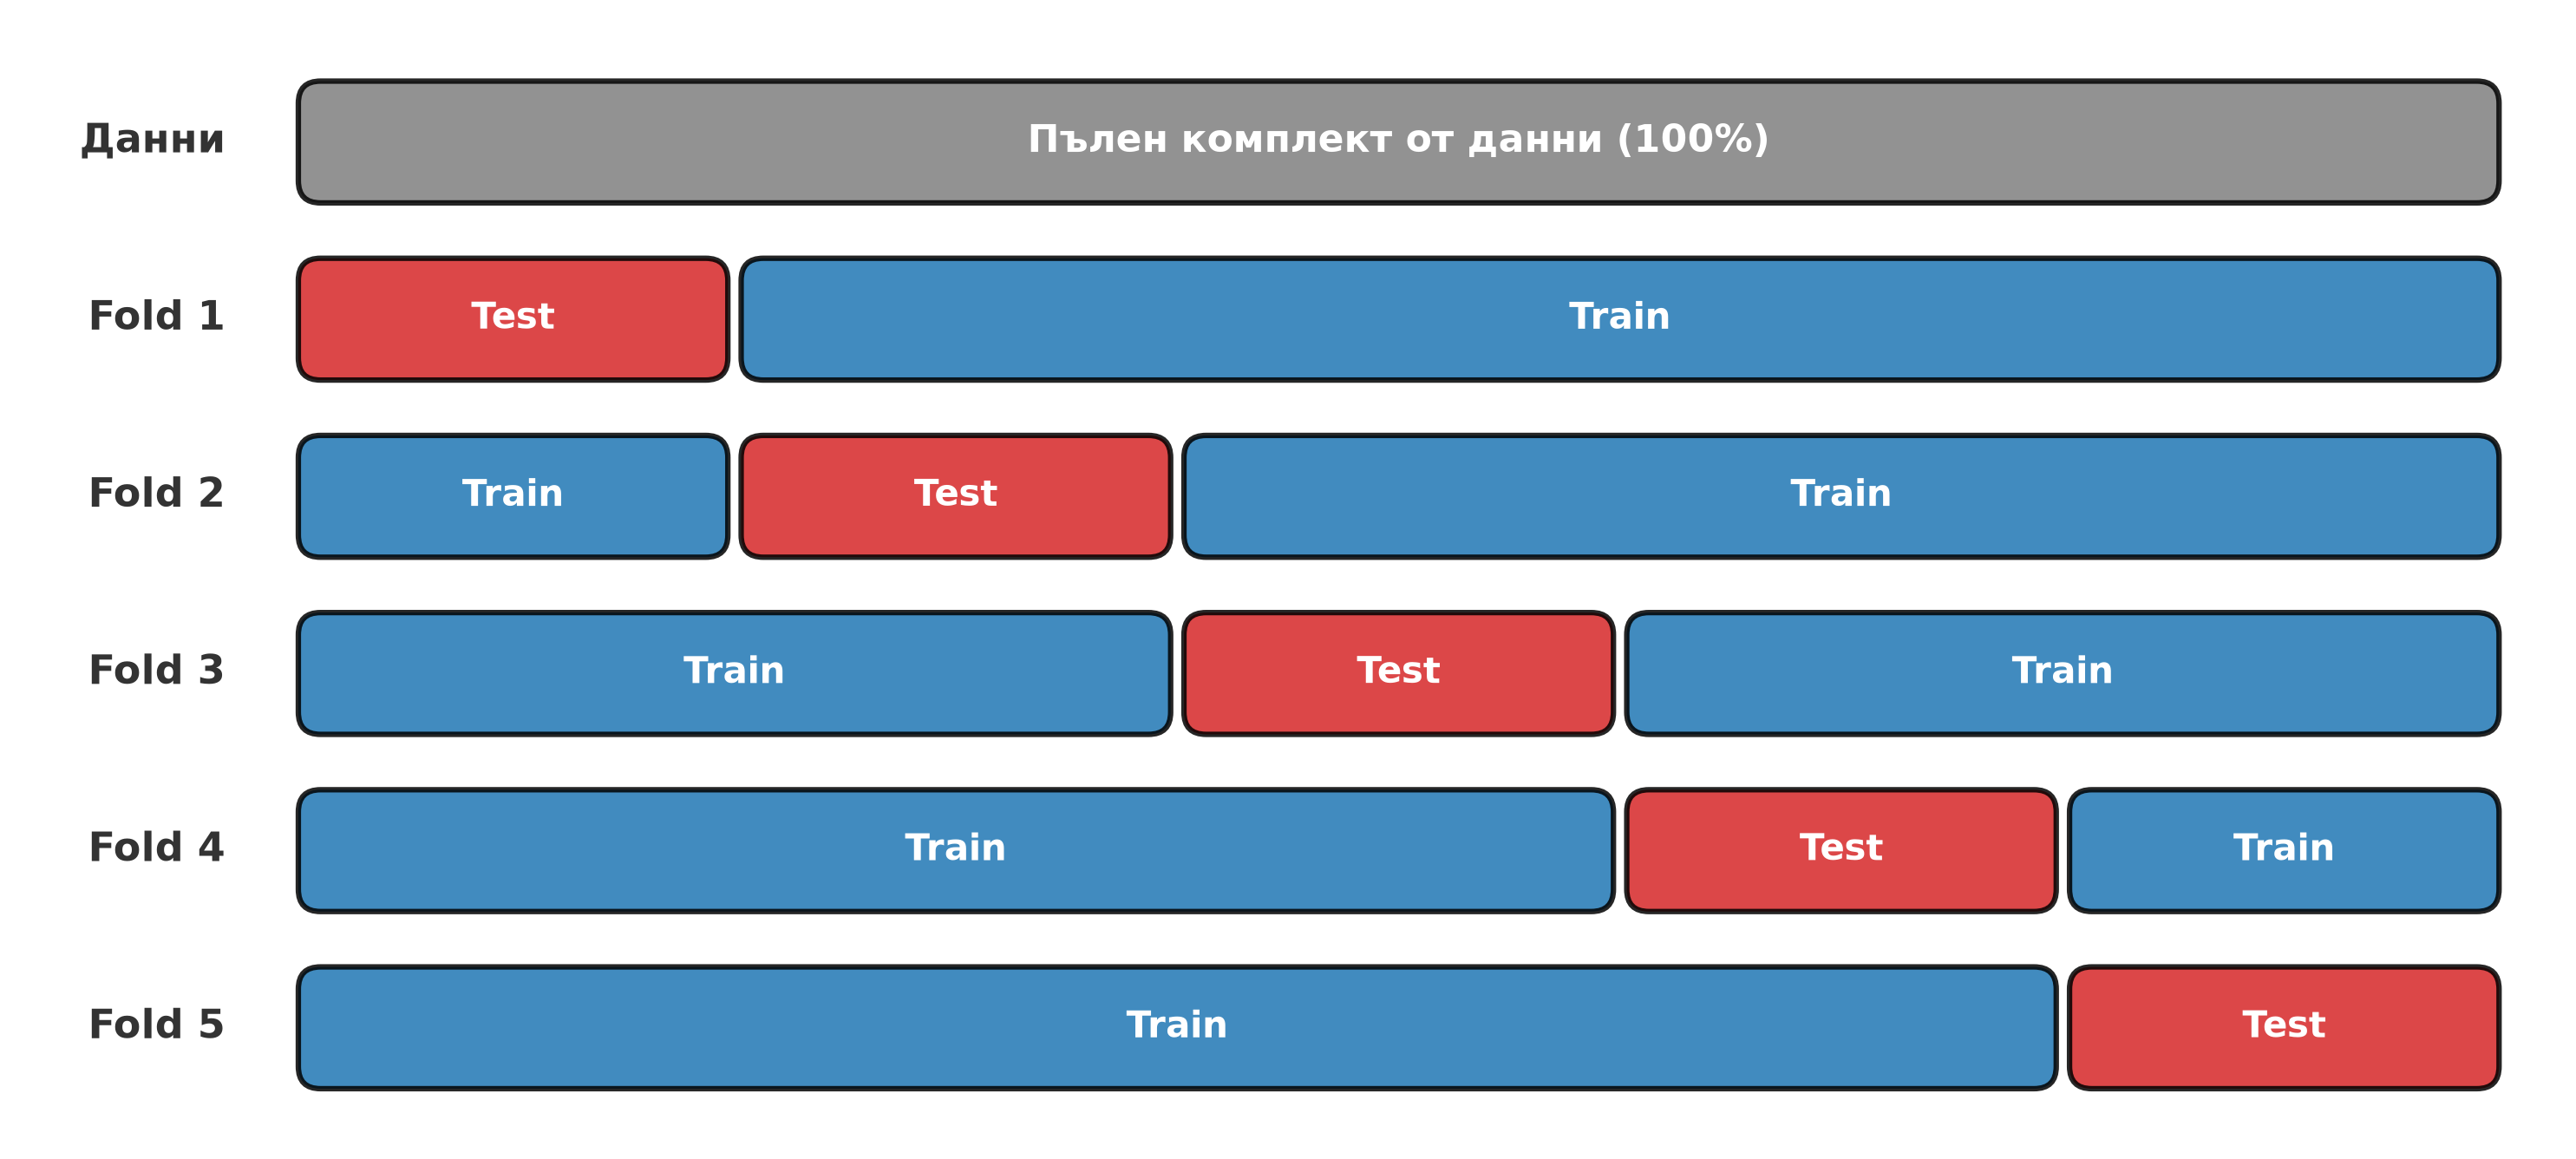
\includegraphics[width=0.7\textwidth]{images/5fold_cross_validation.png}
  \end{itemize}
\end{frame}

% --------------------------------------------------------------------------------

\subsection{Обобщение}

% --------------------------------------------------------------------------------

\begin{frame}
  \begin{itemize}
    \item Каква е разликата между истинската функция и оценената функция?
    \item Какви са компонентите на очакваната грешка?
    \item Защо говорим за баланс между систематична грешка и вариация?
    \item Какво е важно при избора на метрика?
    \item Защо е важно разделянето на данните на тренировъчни и тестови?
  \end{itemize}

\end{frame}
% --------------------------------------------------------------------------------

\end{document}

% --------------------------------------------------------------------------------
